\documentclass[]{article}

\usepackage{amsmath}
\usepackage[a4paper,bindingoffset=0.0in,%
left=0.4in,right=0.4in,top=0.4in,bottom=0.4in,%
footskip=.25in]{geometry}
\usepackage{hyperref}
\usepackage{graphicx}
\usepackage{subcaption}

\graphicspath{ {./results/} }
\hypersetup{
	colorlinks=true,
	linkcolor=blue,
	filecolor=magenta,      
	urlcolor=cyan,
}

%opening
\title{CMPT469 Final Project - Image Alignment and Stitching}
\author{Curtis Buckoll - 301291952}

\begin{document}

\maketitle

% -----------------------------------------------------------------------

\vspace{5mm}
\textbf{1) The Problem}
\vspace{3mm}

The focus of this project is the explore the techniques used in image alignment and stitching, that is, given a set of images featuring a common scene, how do we best fit them together? We want to develop a process to produce the results as demonstrated in the following figures

\begin{figure}[h]
	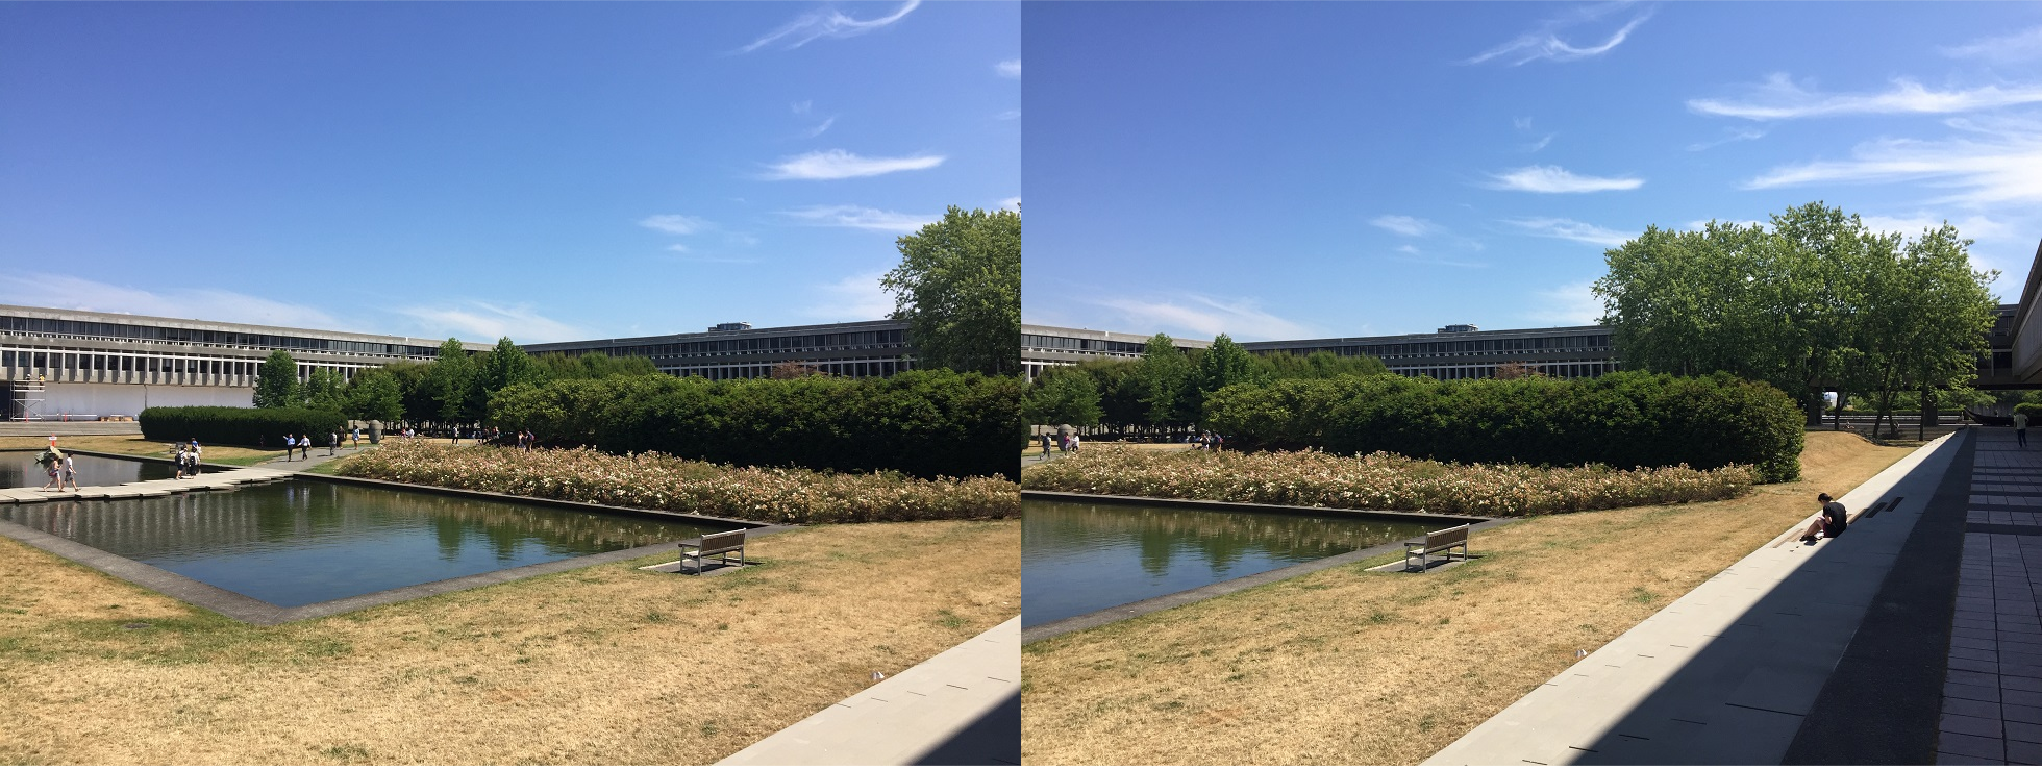
\includegraphics[scale=0.55]{results/p1_noblend/1}
	\centering
	\caption{Images A, B}
\end{figure}
\begin{figure}[h]
	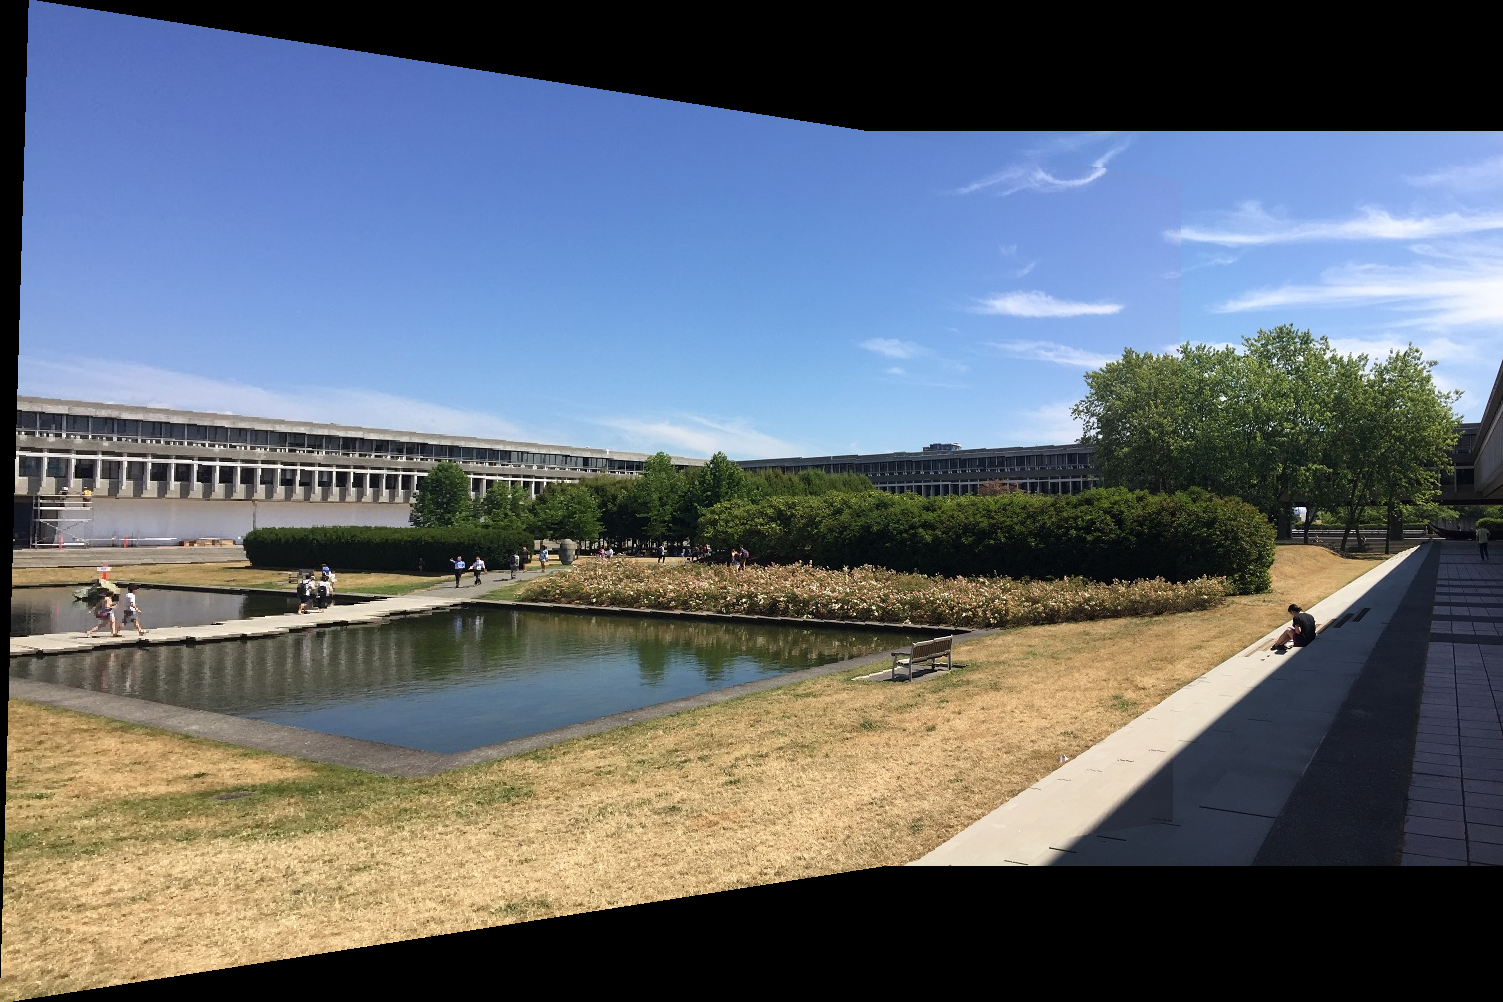
\includegraphics[scale=0.25]{results/p1_noblend/4}
	\centering
	\caption{Image A and B fit together}
\end{figure}

\noindent There are a number of sub-problems in the pipeline, consisting of the following steps: \\

1) Given two images, detect points of interest and compute their SIFT descriptors.

2) Amongst these points, compute ‘ratio scores’ to determine the most promising feature matches between images

3) Perform RANSAC and obtain a refined subset of matches from which to compute a homography.

4) Project one image onto the other and blend. \\

Detecting interest points can be done by the Harris corner algorithm. For these interest points, we can then can then compute their SIFT descriptors describing gradient information local to each point. In this implementation, vl{\_}sift() from the VLFEAT bundle was used to both find interest points and get their descriptors. We can compare the similarity of two descriptors simply by taking their sum of square difference score, and we use the ratio test to create correspondences between interest points from both images. This works just as studied: for all points in image A, find it's closest and second closest matches in image B. The ratio score for that pairing is the SSD of the best match divided by the SSD of the second best, where anything with a score below 0.7 was accepted. This procedure worked quite reliably. We can see from the following image depicting the ratio-tested feature matches that while there are some evident outliers, there is also quite a strong correspondence of correct matches.

\begin{figure}[h]
	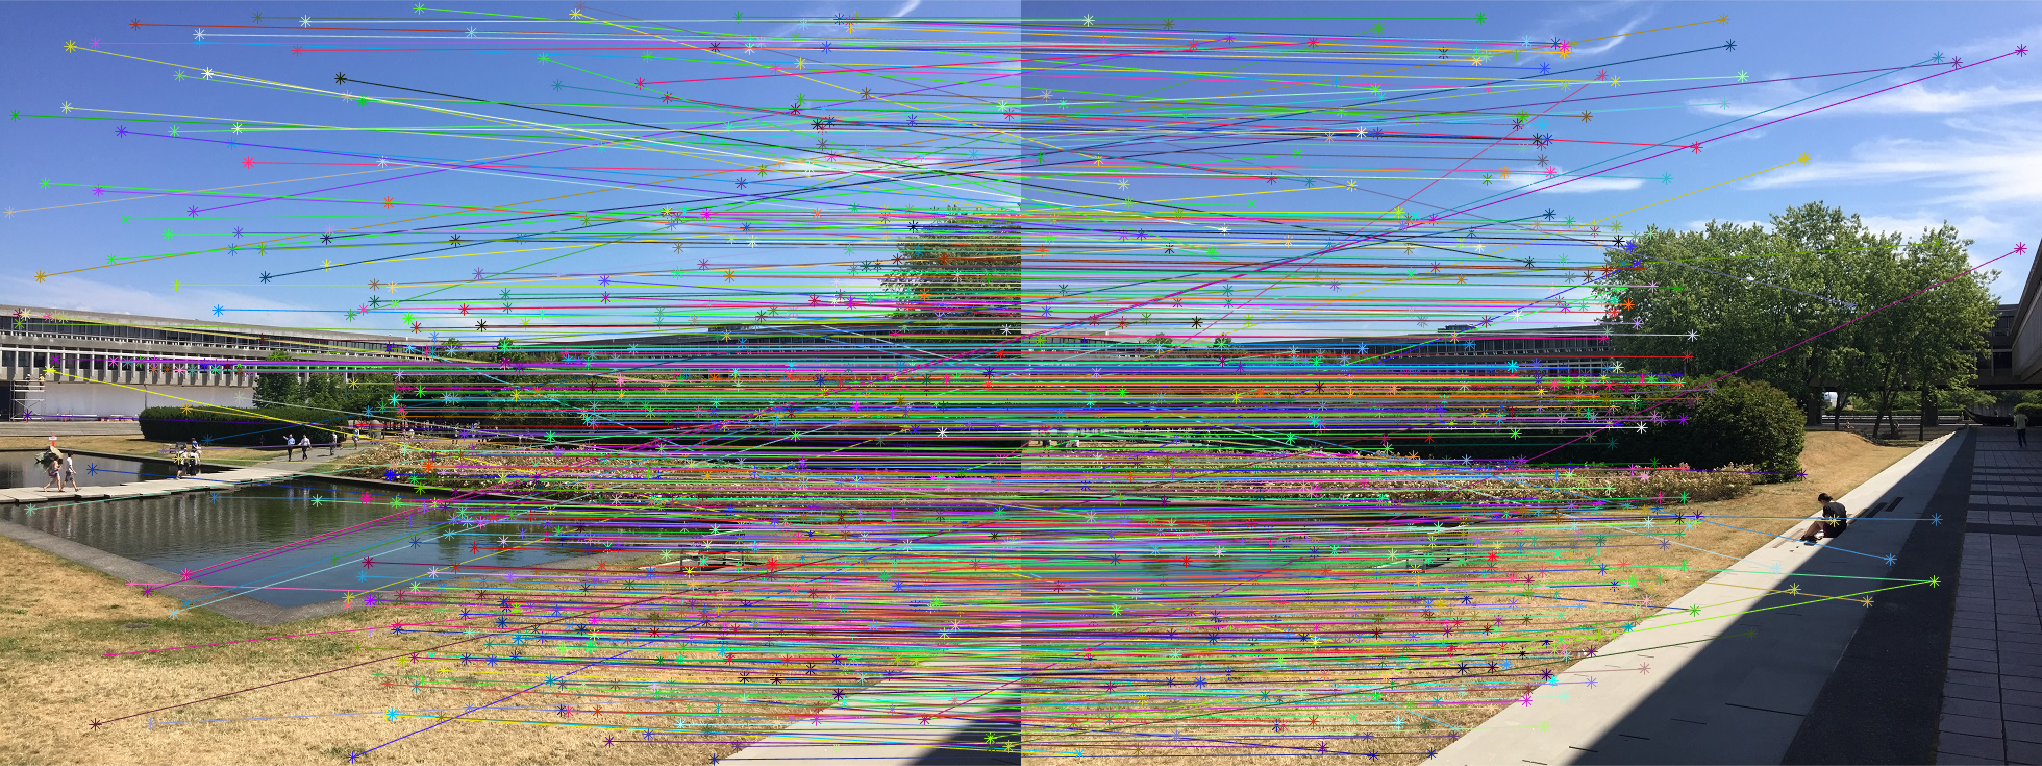
\includegraphics[scale=0.55]{results/p1_noblend/2}
	\centering
	\caption{The supposed matches found by the ratio test}
\end{figure}

At this point, although there could be many correct feature matches, we do not inherently know which ones are correct and which ones are not. So to move forward, we take these pairings and perform RANSAC to obtain a most-trusted subset of matches from which we can compute a homography. In this implementation, the RANSAC algorithm was adopted in the following way: amongst all feature matches obtained from the ratio test, pick four matches at random and compute a homography H. We choose four points, as this is the minimum number needed to obtain a homography. Then, all coordinates from Image A are transformed by H, and we observe how 'close' they end up to their supposed image B pairings. We use Euclidean distance in terms of pixels to gauge the result, where it was found through experimentation that a radius of 3 pixels worked well as a threshold. If the threshold were any higher, we would occasionally be mistaking outliers for inliers, skewing the final transformation. Conversely, if the threshold were set too small, then we would sometimes end up with too few matches to get any result. This procedure was repeated some number of times, counting the number of inliers produced at each iteration. At the end, the feature matches found from the iteration that produced the most inliers were taken to compute a final homography $H^\prime$, and this was our approximated mapping for image A onto image B.

\begin{figure}[h]
	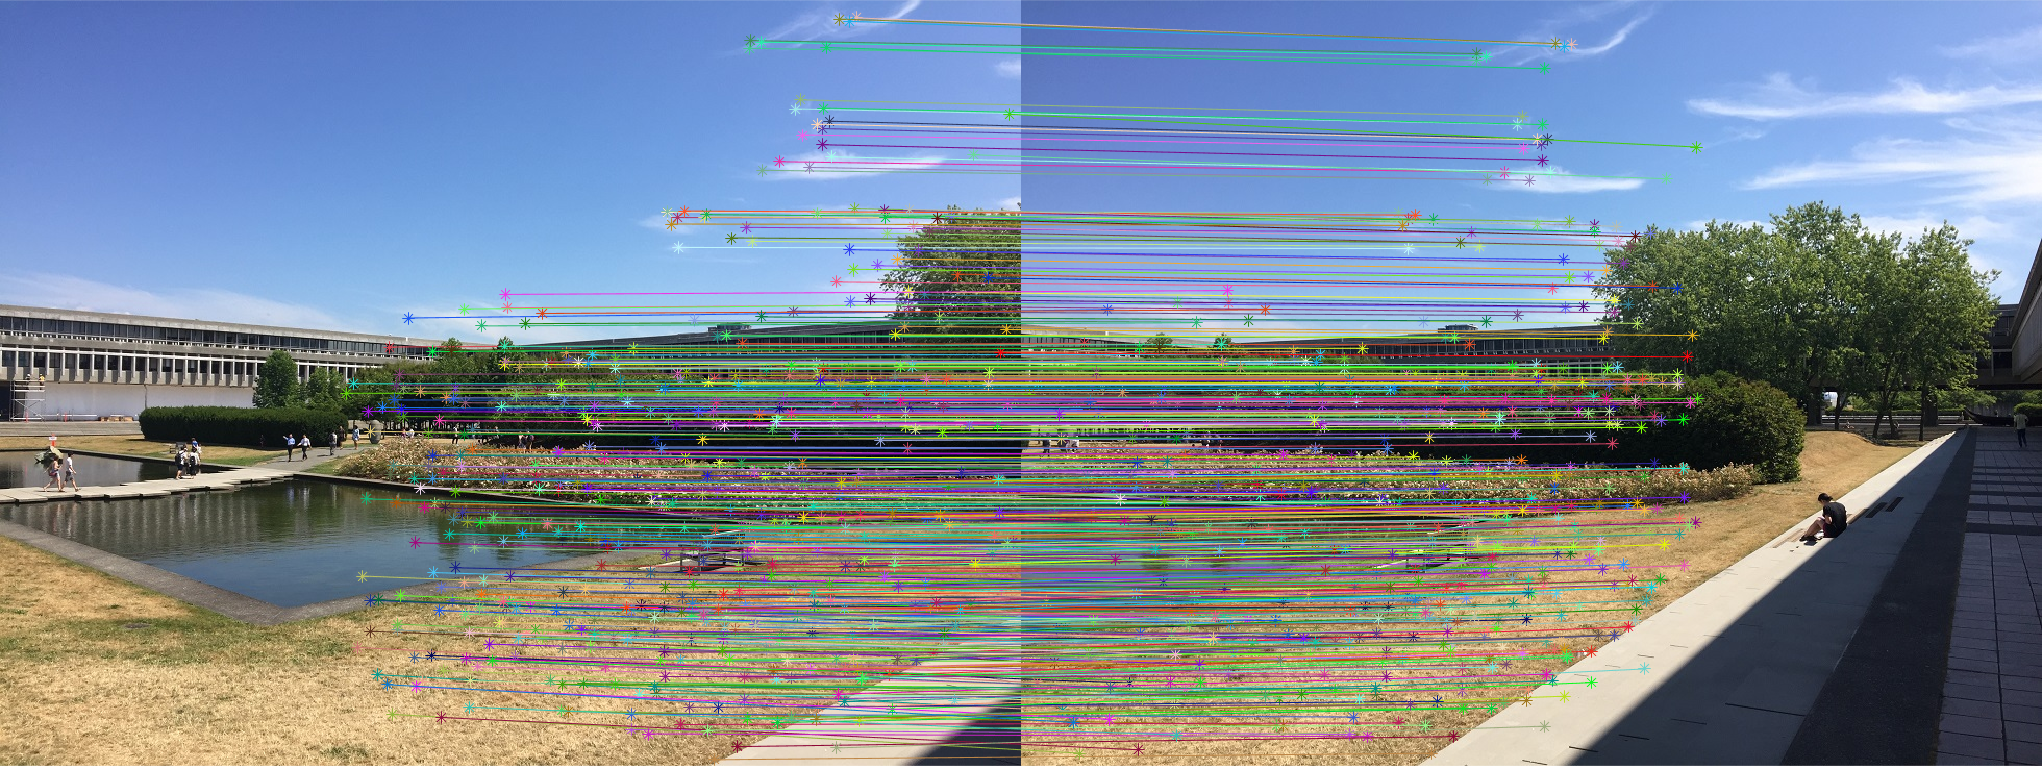
\includegraphics[scale=0.55]{results/p1_noblend/3}
	\centering
	\caption{The largest subset of inliers found by RANSAC}
\end{figure}

This approach is non-deterministic due to the random nature of selecting points, and in fact, running RANSAC on the same two images would occasionally produce very minutely different results. But given enough iterations, some acceptable result was always found. Initially, this implementation allowed for 500 iterations, which seemed fairly stable. This was later increased to 2000, which seemed quite sufficient. However, there did not appear to be a significant performance hit for further increasing this number, and so eventually 10000 iterations were allowed. Of course, the number of iterations required is entirely dependent on the initial number of feature matches found along with the proportion of correct matches, but for all test images that were tried, 10000 iterations seemed to be more than enough.

With everything in place to project the image, we inversely map pixels from image A onto B by  $H^{\prime-1}$, and we obtain the desired result:

\begin{figure}[h]
	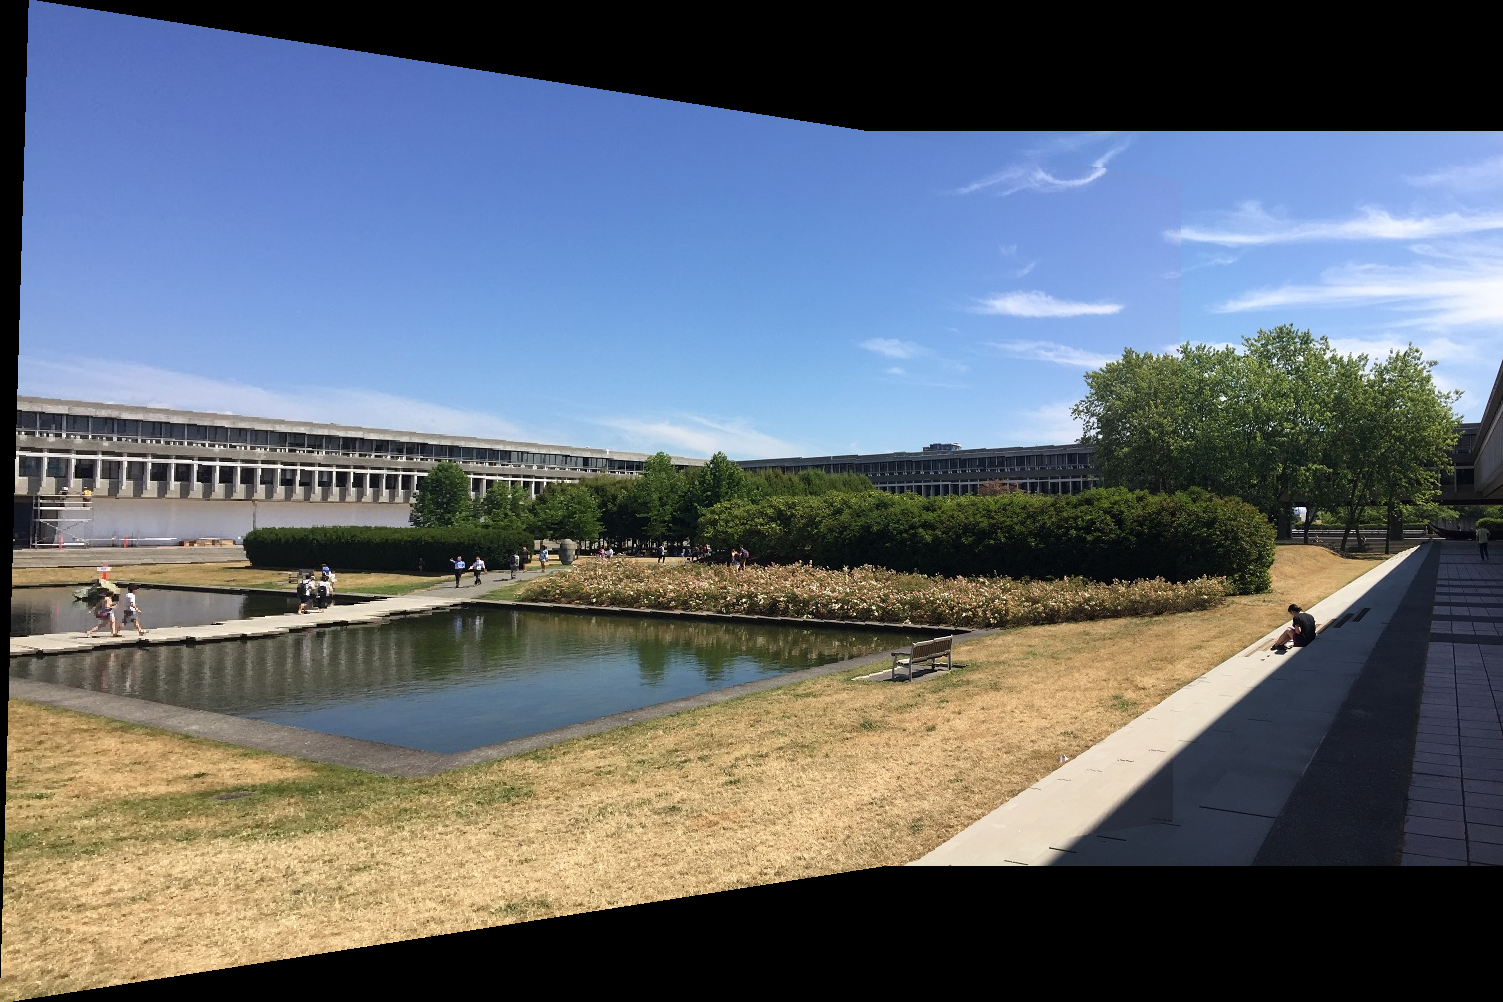
\includegraphics[scale=0.23]{results/p1_noblend/4}
	\centering
	\caption{Image A aligned and projected onto image B}
\end{figure}

From here, we can simply repeat the same process with more images,

\begin{figure}[h]
	\begin{subfigure}[h]{0.5\textwidth}
		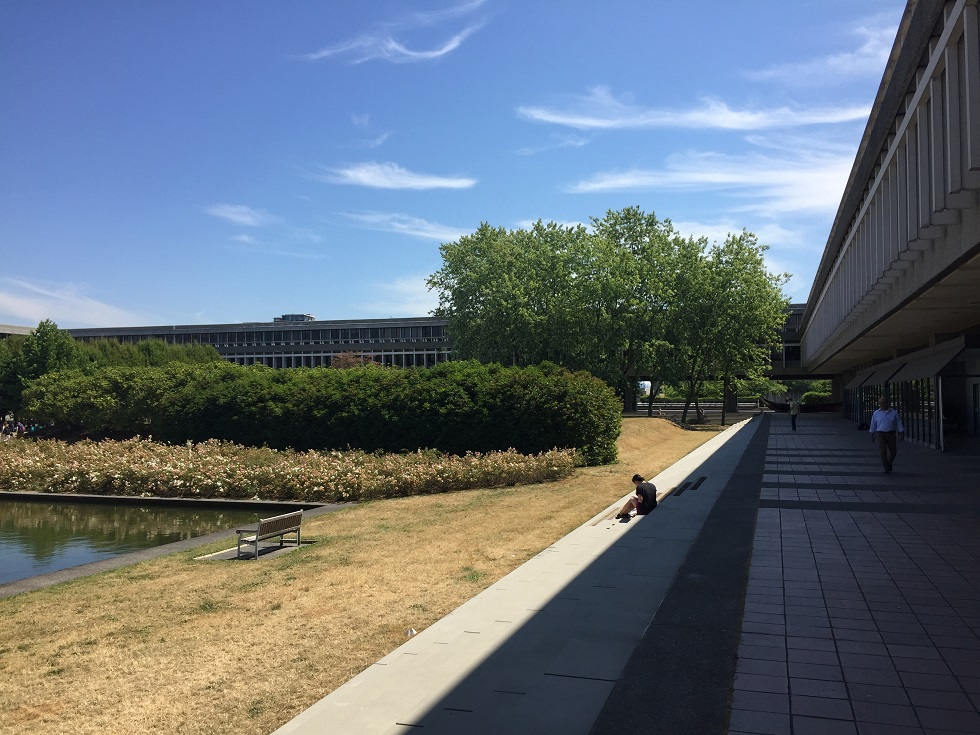
\includegraphics[scale=0.25]{results/p1_noblend/C}
		\centering
		\caption{Image C}
	\end{subfigure}%
	\hfill
	\begin{subfigure}[h]{0.5\textwidth}
		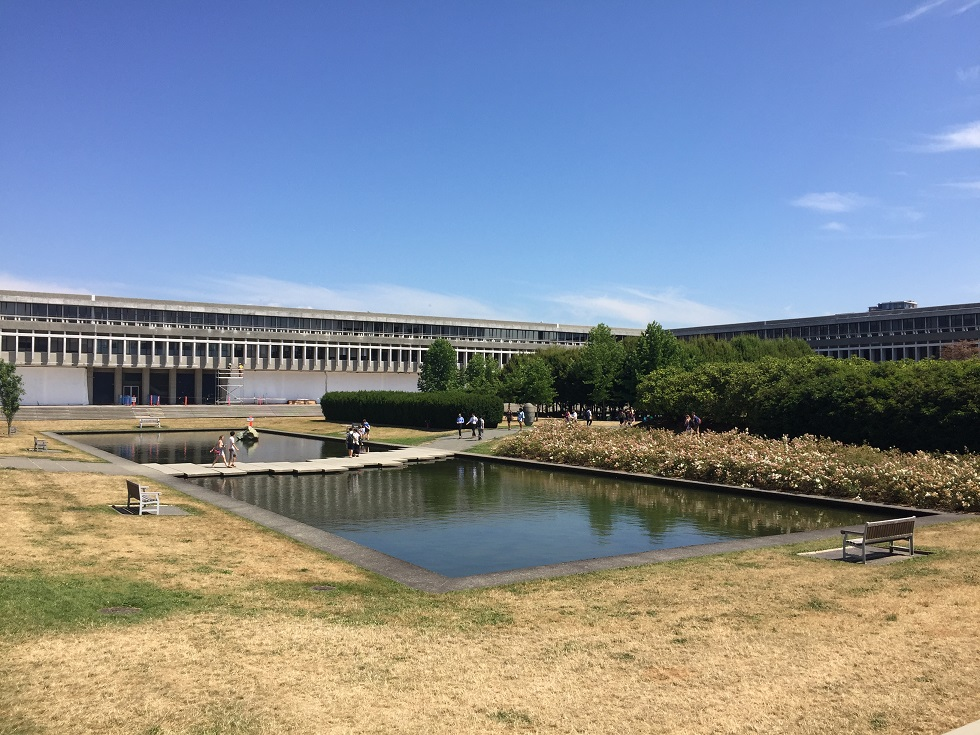
\includegraphics[scale=0.25]{results/p1_noblend/D}
		\centering
		\caption{Image D}
	\end{subfigure}%
	\centering
\end{figure}
\begin{figure}[h]
	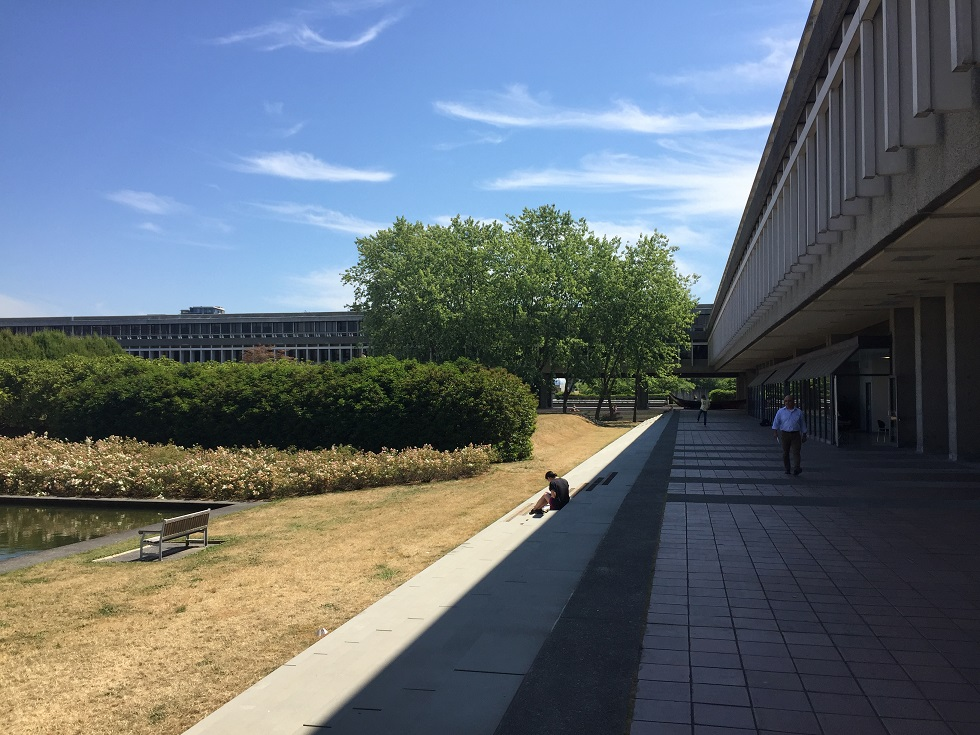
\includegraphics[scale=0.25]{results/p1_noblend/E}
	\centering
	\caption{Image E}
\end{figure}

And we get the final five-image composite of images A, B, C, D, E:
\vspace{30mm}

\begin{figure}[h]
	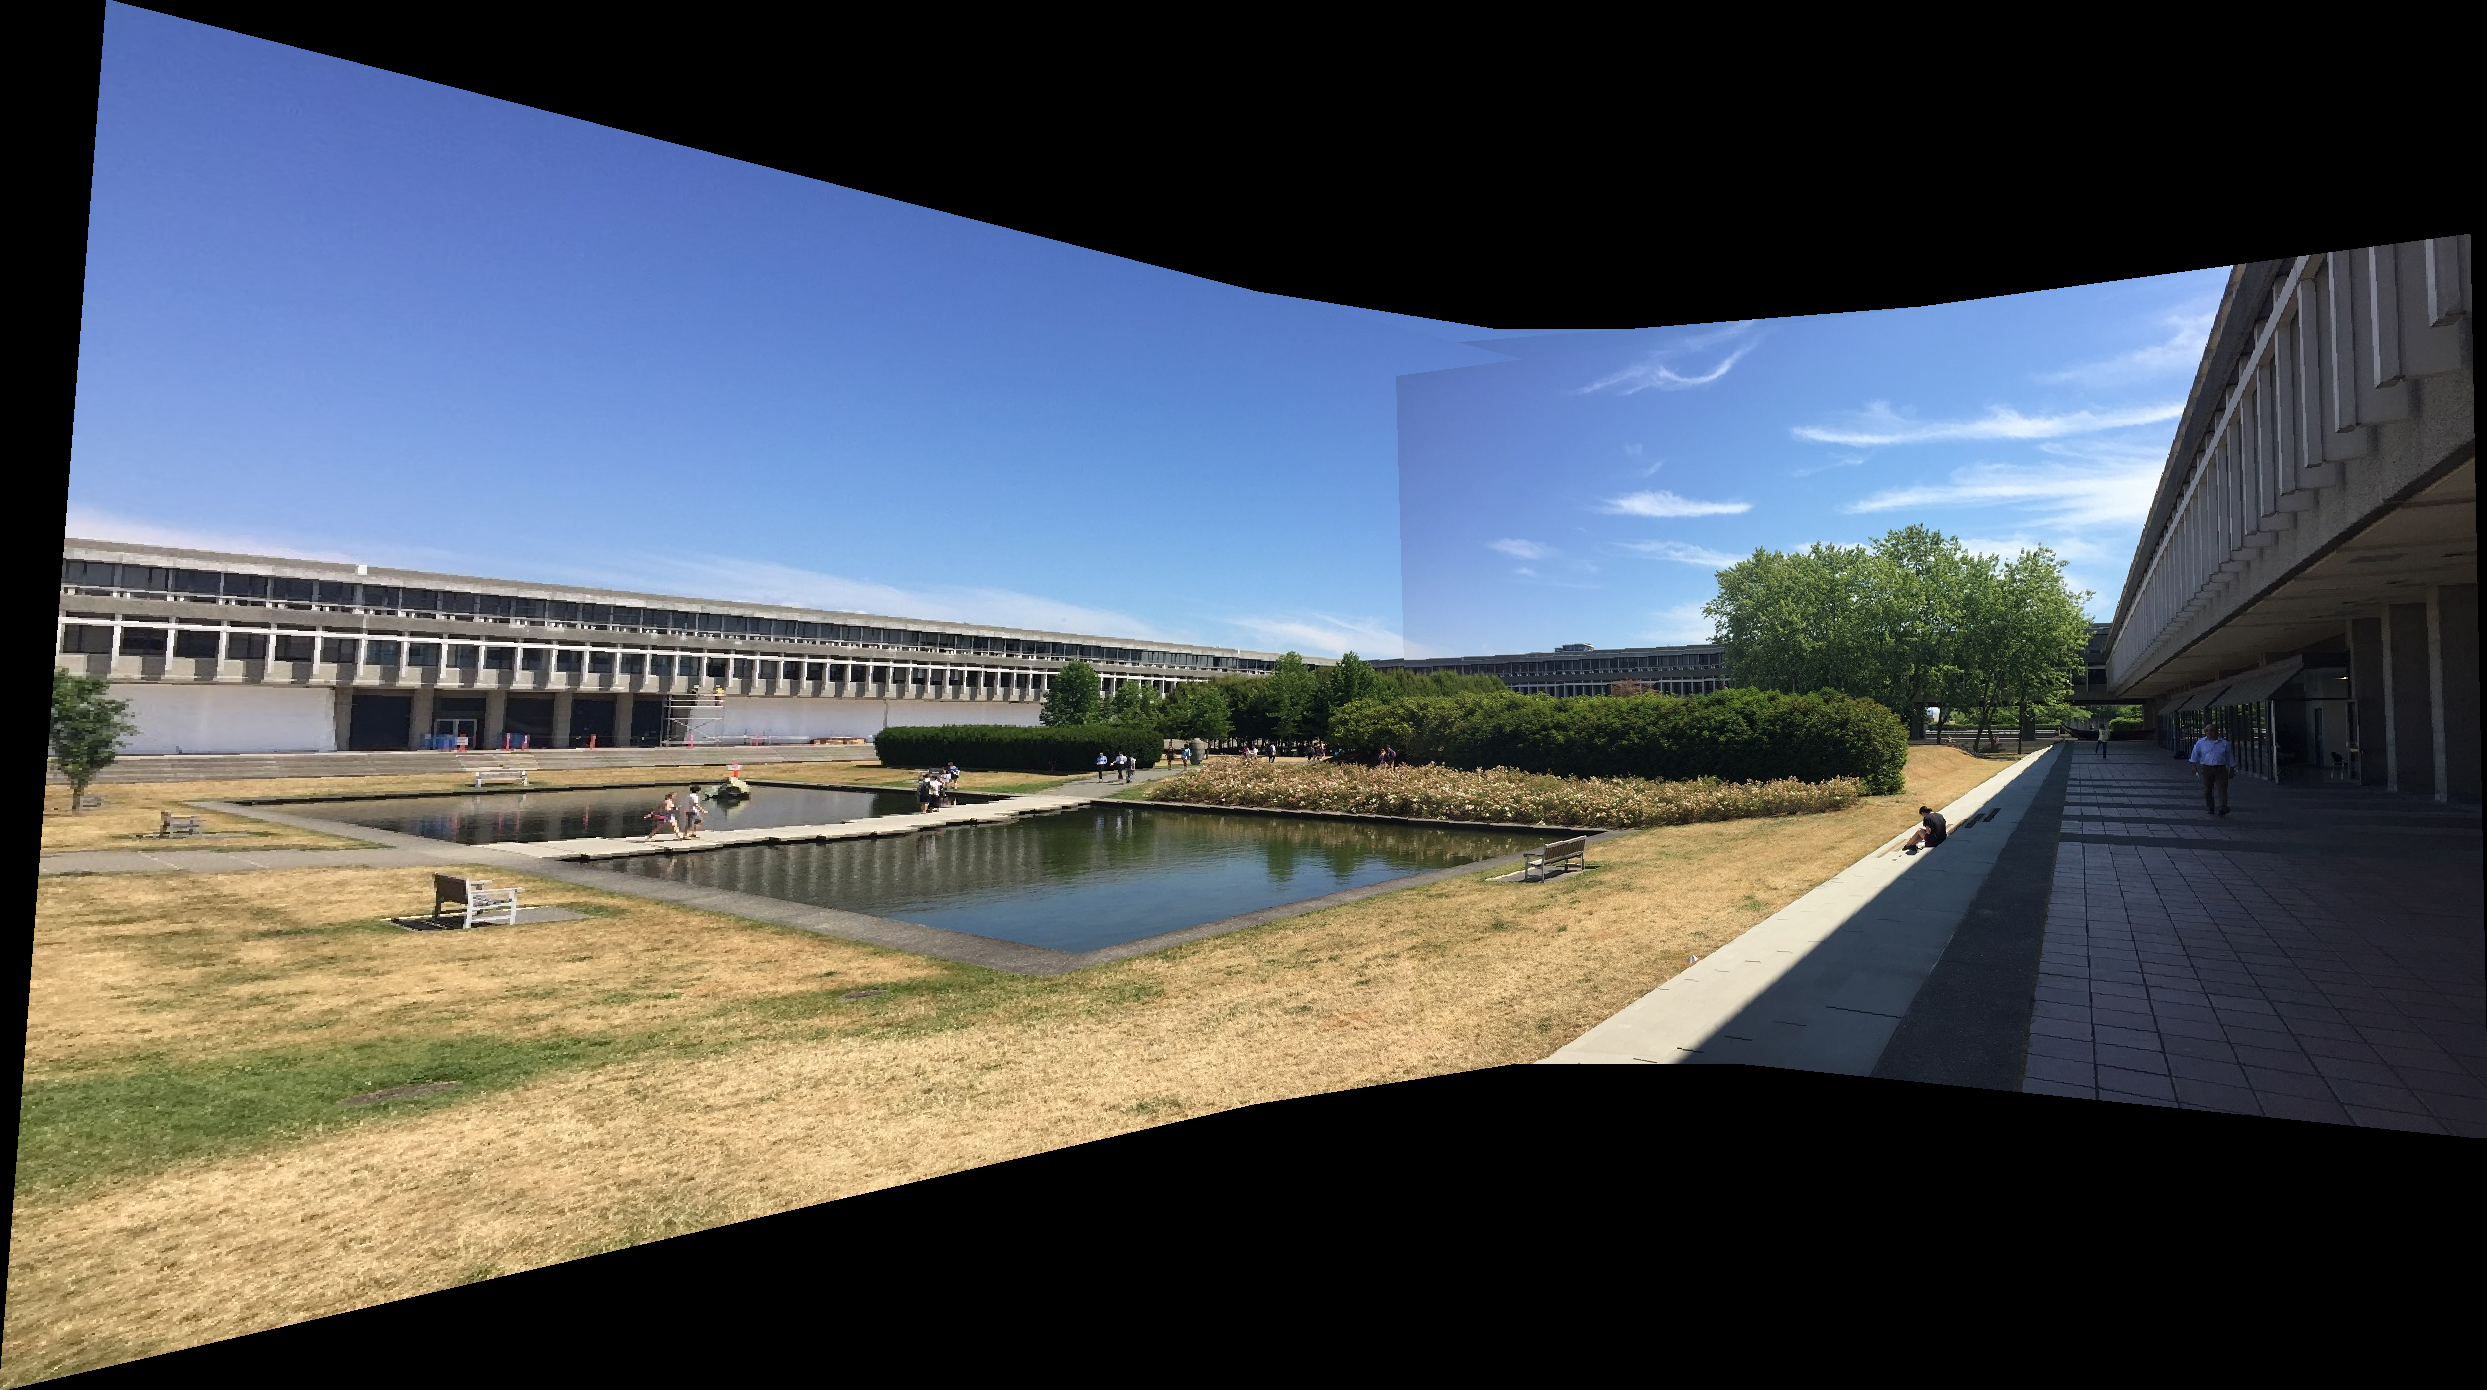
\includegraphics[scale=0.2]{results/p1_noblend/16}
	\centering
	\caption{Five-image composite}
\end{figure}

At this point, it remains to blend the stitched images into a single seamless result. The blending approach was arrived at with some experimentation, and it combined two-band blending and feathering techniques. First, the overlapping portions of the image were split into their low and high frequency components, and then these components were blended over different curves. The low frequency component was blended smoothly over a gentle curve, and the high frequency component was blended over a sharper one. Both curves were based on the sigmoid function, and were found by experimenting with different image results.

\begin{align*}
\textrm{High Frequency Curve: }&\frac{1}{e^{-30(\alpha-0.5)} + 1} \\
\textrm{Low Frequency Curve: }&\frac{1}{e^{-10(\alpha-0.5)} + 1}
\end{align*}

\begin{figure}[h]
	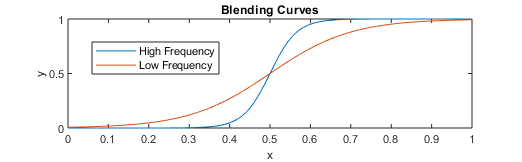
\includegraphics[scale=1]{results/blending_curves}
	\centering
	\caption{The low and high-frequency blending curves parameterized by $\alpha \in [0,1]$}
\end{figure}

This allowed smooth transitions in the low frequency to come together in a pleasing way, while applying a better suited transition to the sharper detail of the high frequency channel that reduced subtle detail conflicts. This arrives us at our final blended panorama image,
\vspace{50mm}

\begin{figure}[!h]
	\includegraphics[scale=0.2]{results/p1_blend/16}
	\centering
	\caption{Five-image blended composite}
\end{figure}

\noindent along with one other good result, again stitched from five separate images:

\begin{figure}[!h]
	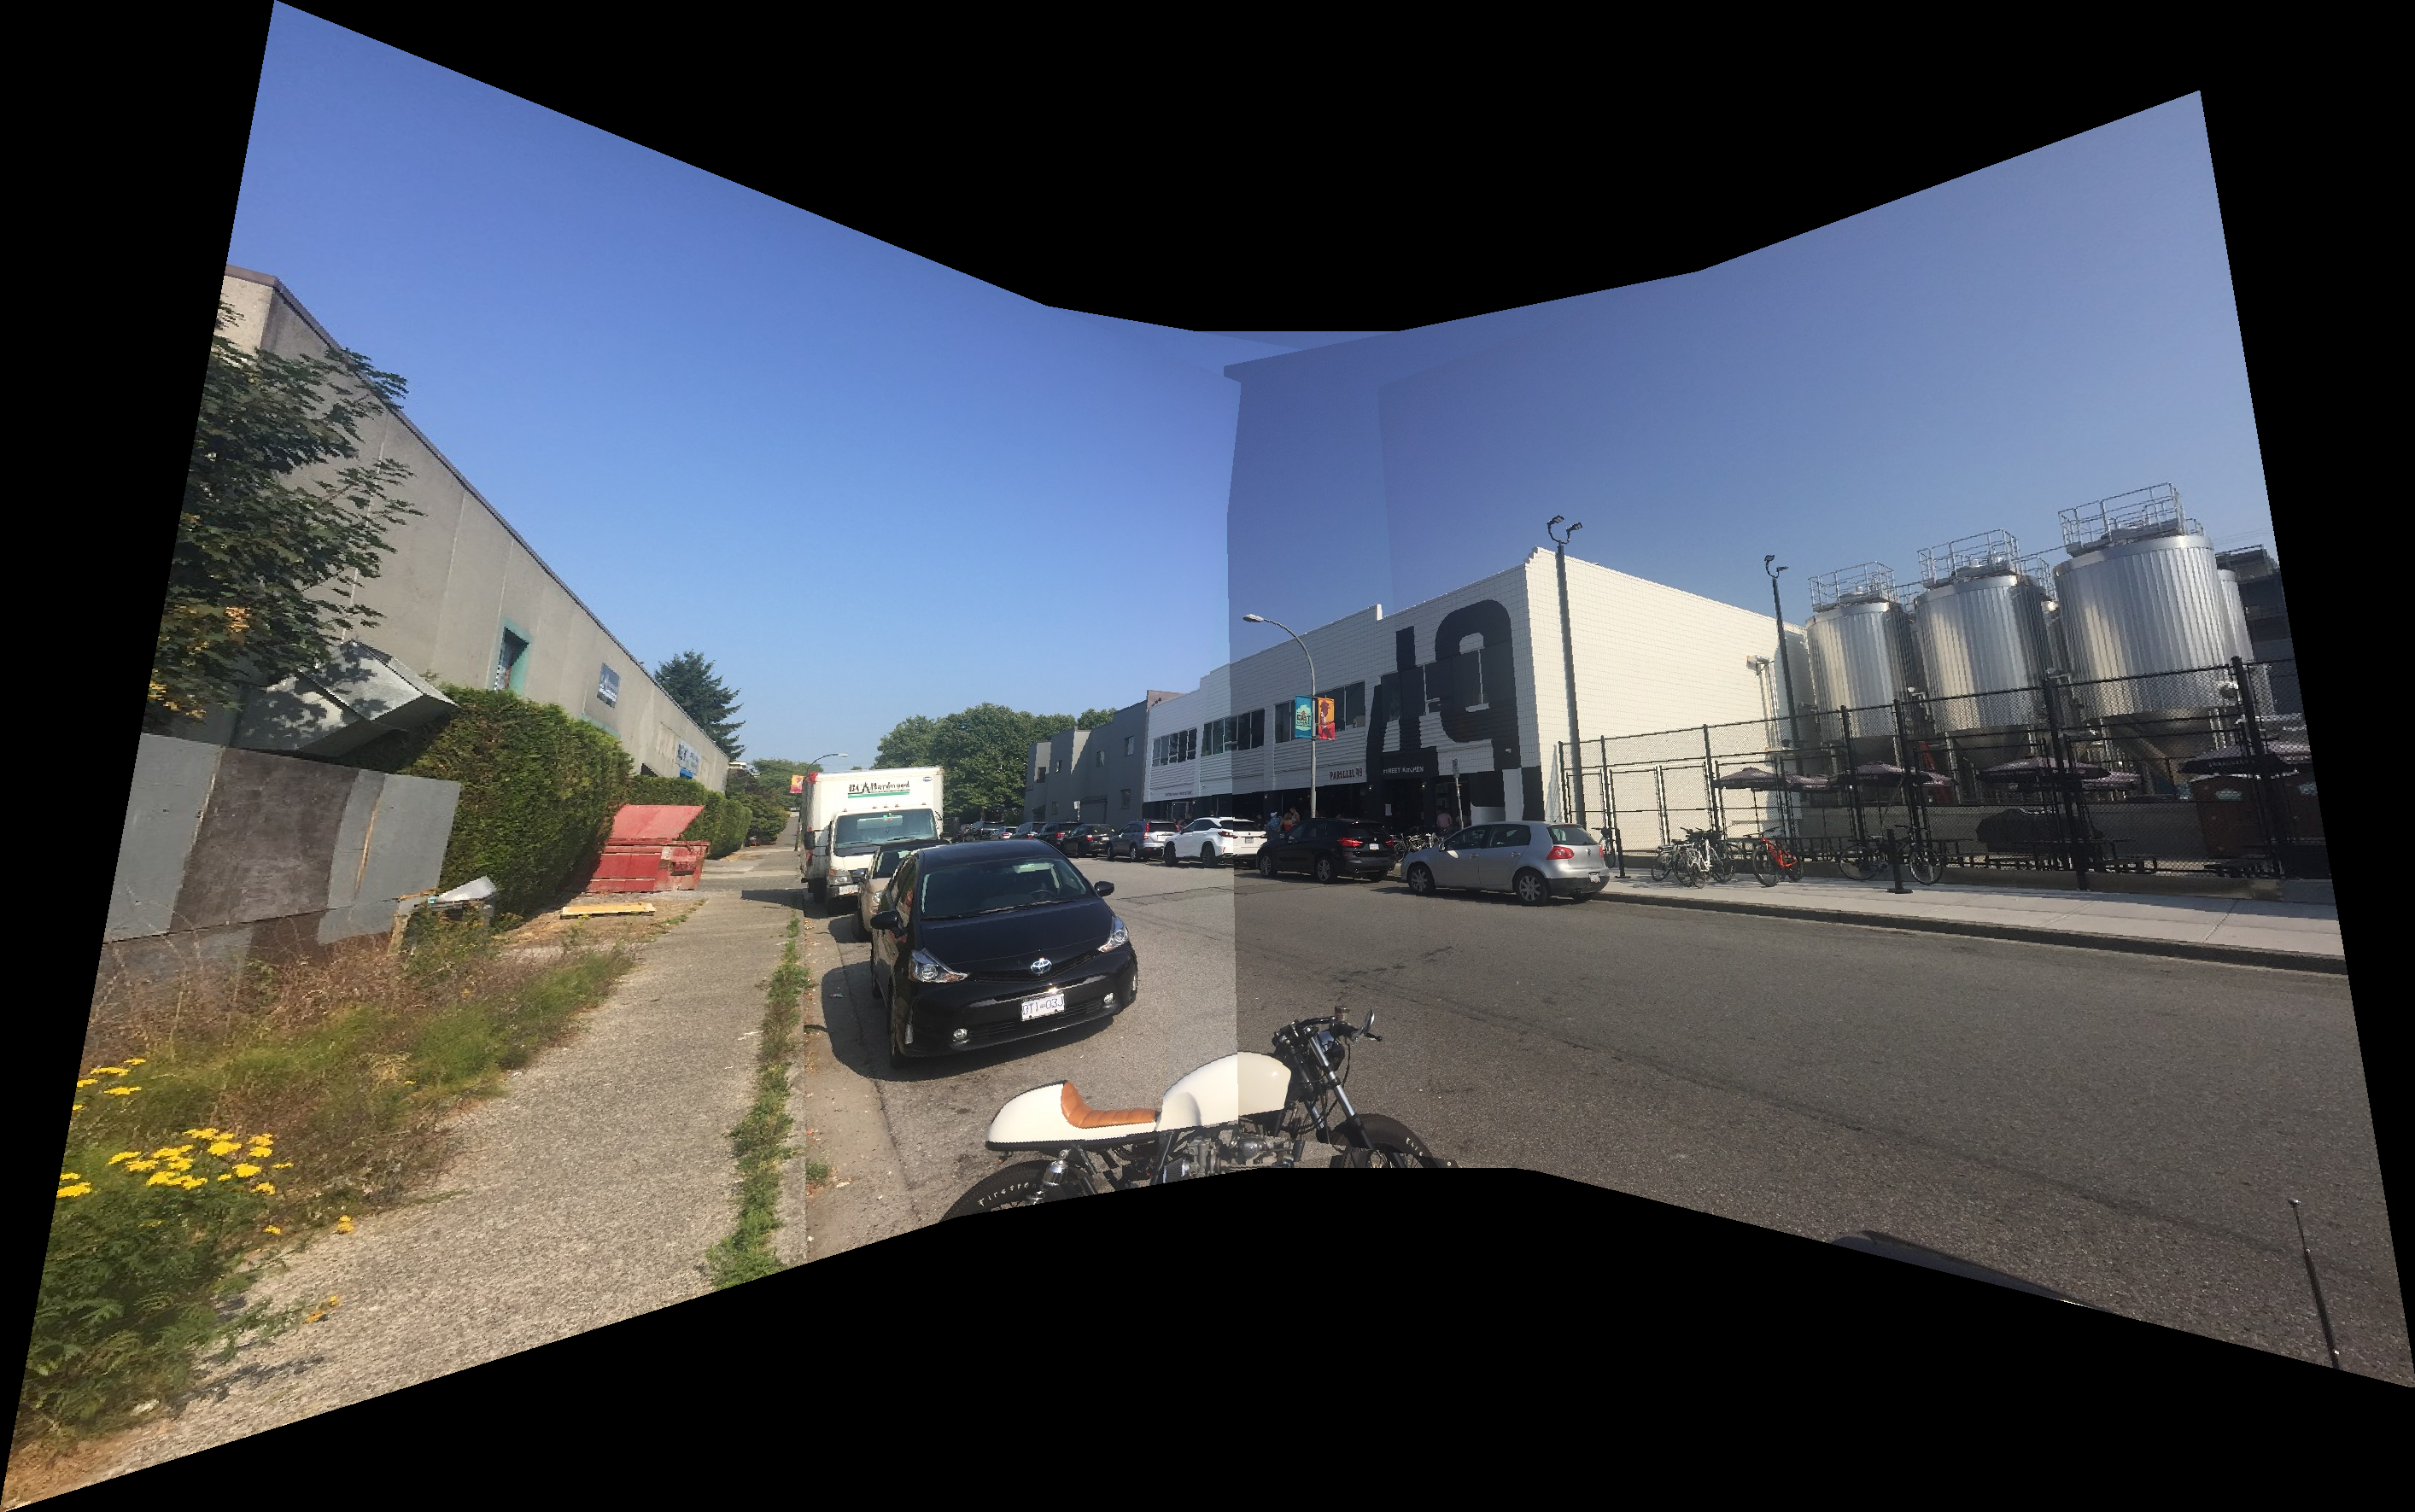
\includegraphics[scale=0.18]{results/p6_noblend/16}
	\centering
	\caption{Another five-image composite}
\end{figure}

\vspace{100mm}

\begin{figure}[h]
	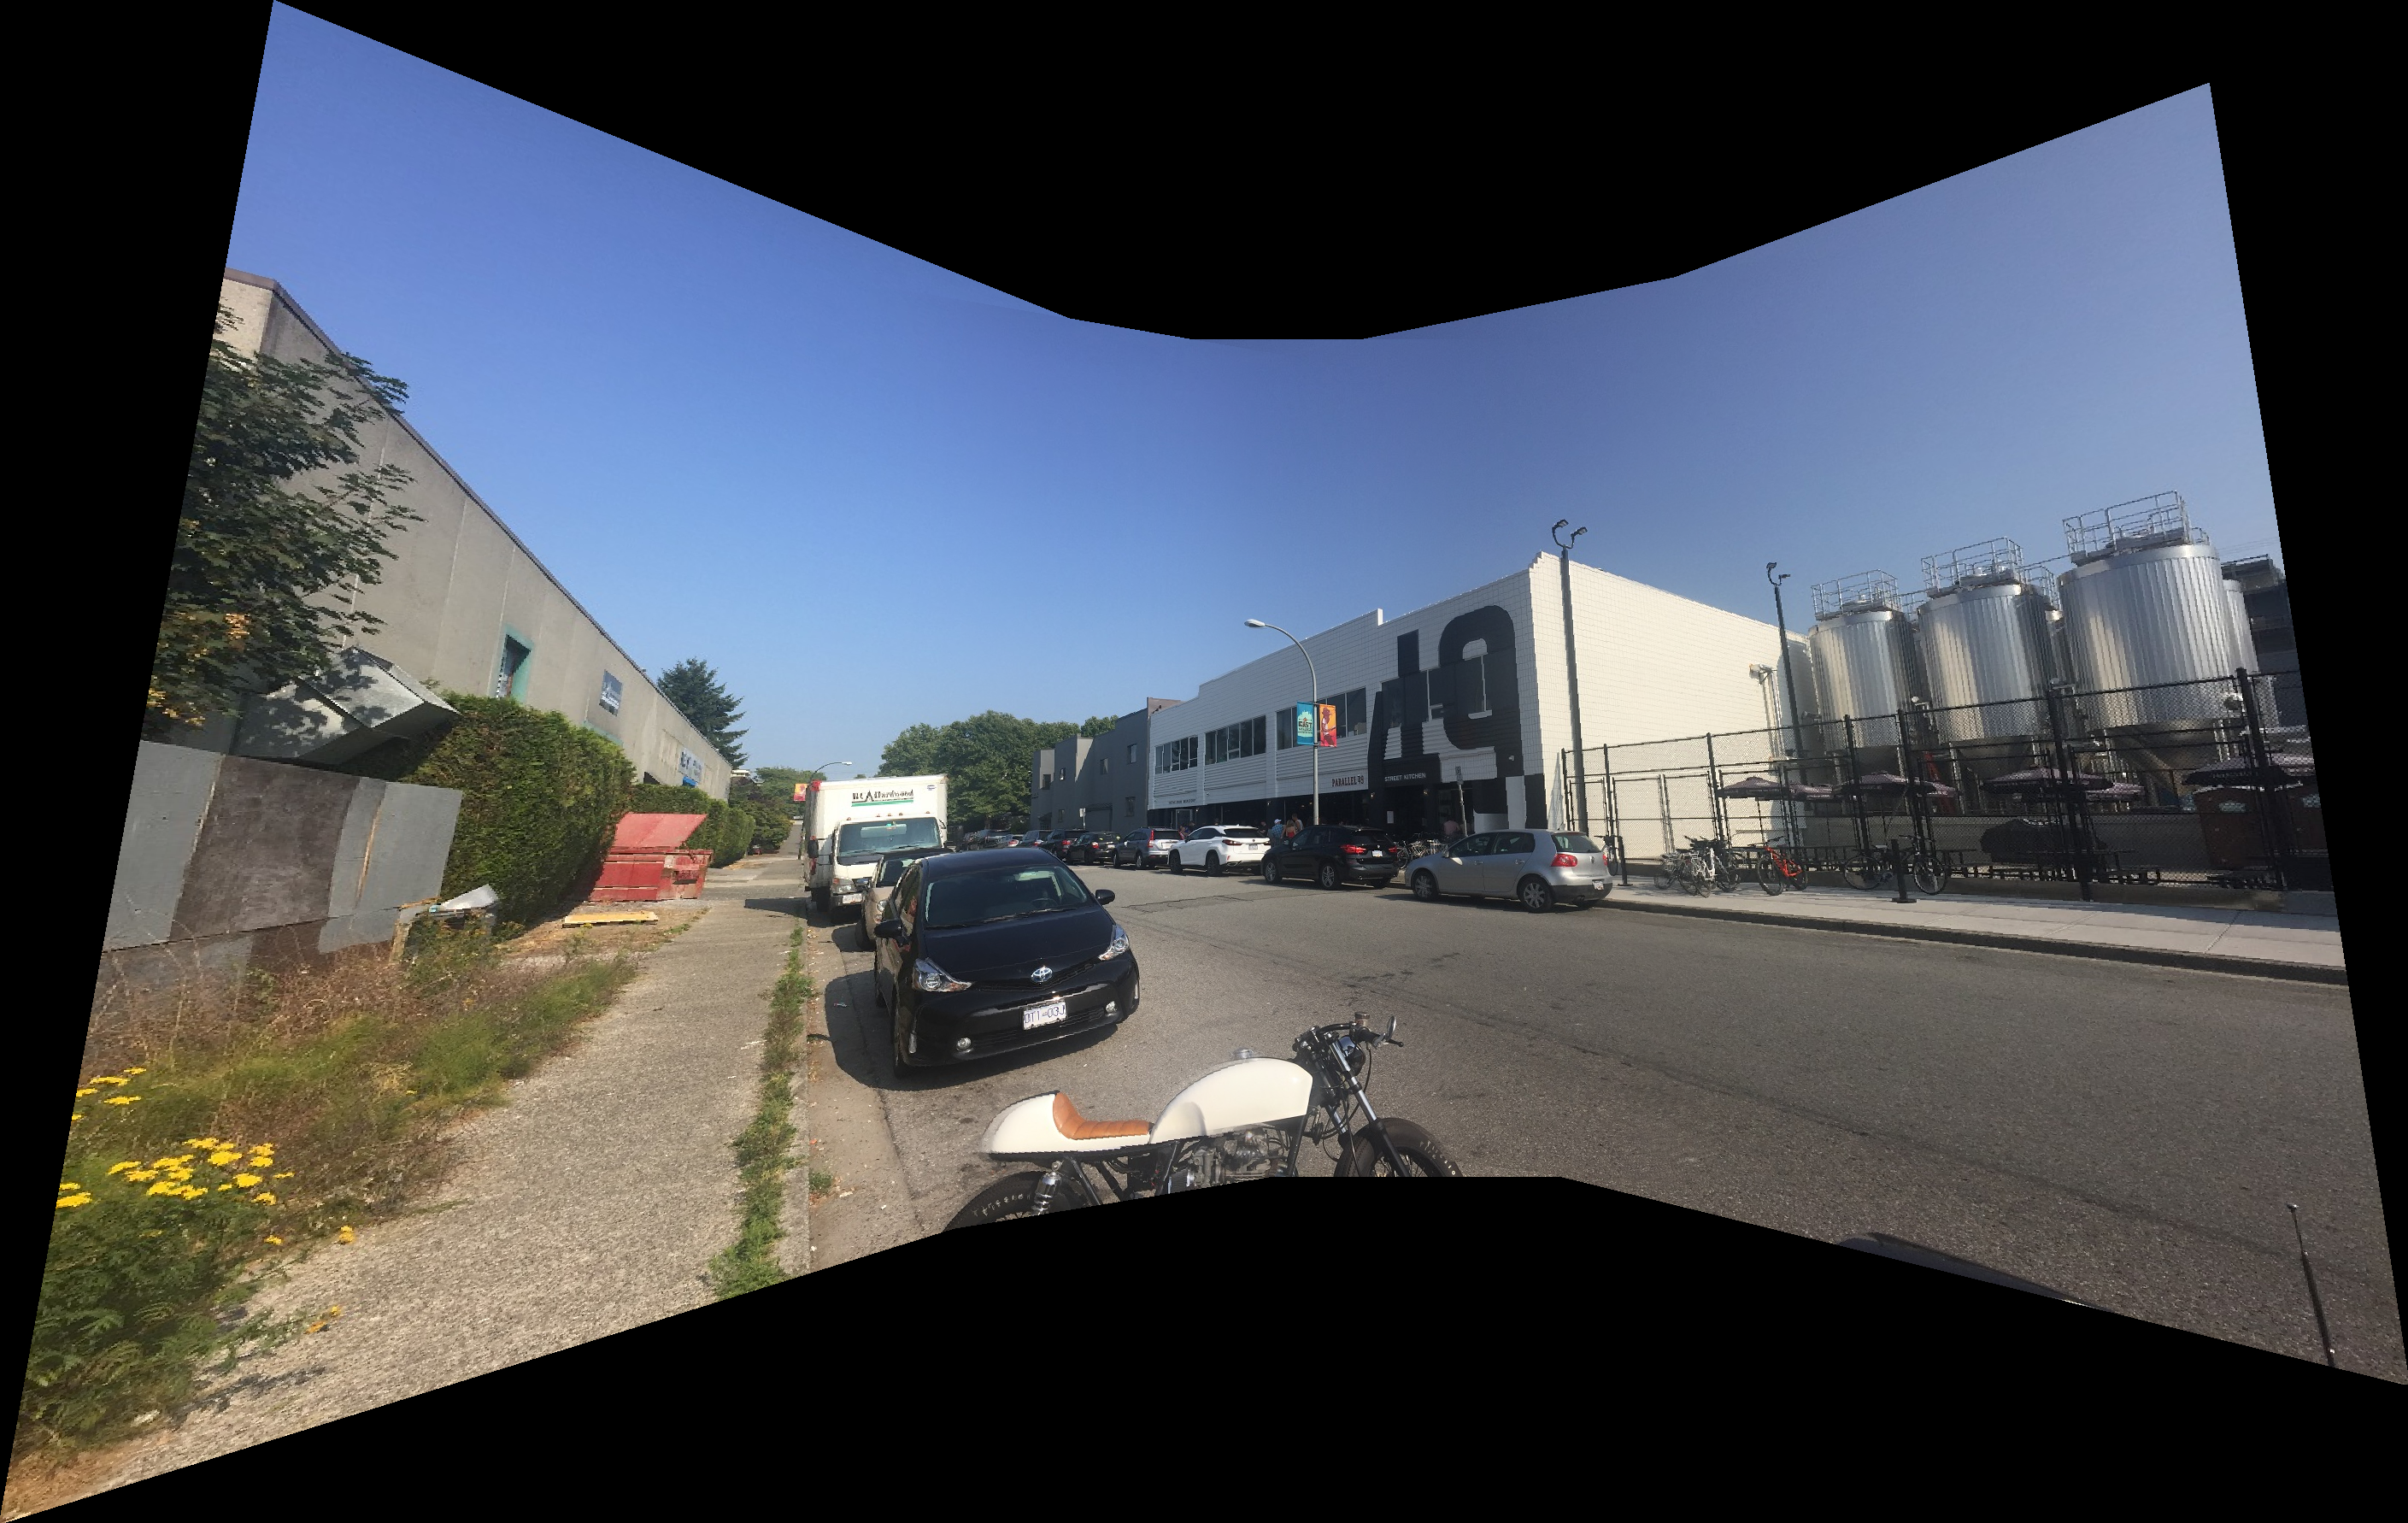
\includegraphics[scale=0.18]{results/p6_blend/16}
	\centering
	\caption{The composite with blending}
\end{figure}

\vspace{30mm}

\vspace{5mm}
\textbf{2) Observations}
\vspace{3mm}

One drawback of the chosen blending strategy is that it requires images that align in a horizontal orientation, and in addition, it only considers the overlapping regions of the images. Because of this, it is possible to end up with small fragments in the composite image that should be blended, but are not. The blending strategy also depends on the images being well-aligned, and can produce 'ghosting' artifacts otherwise. To handle the more general case, gradient domain blending or seam finding might be better alternatives. To demonstrate some of these issues, we can try to align the following five images that do not come together in a horizontal orientation.

\begin{figure}[h]
	\begin{subfigure}[h]{0.2\textwidth}
		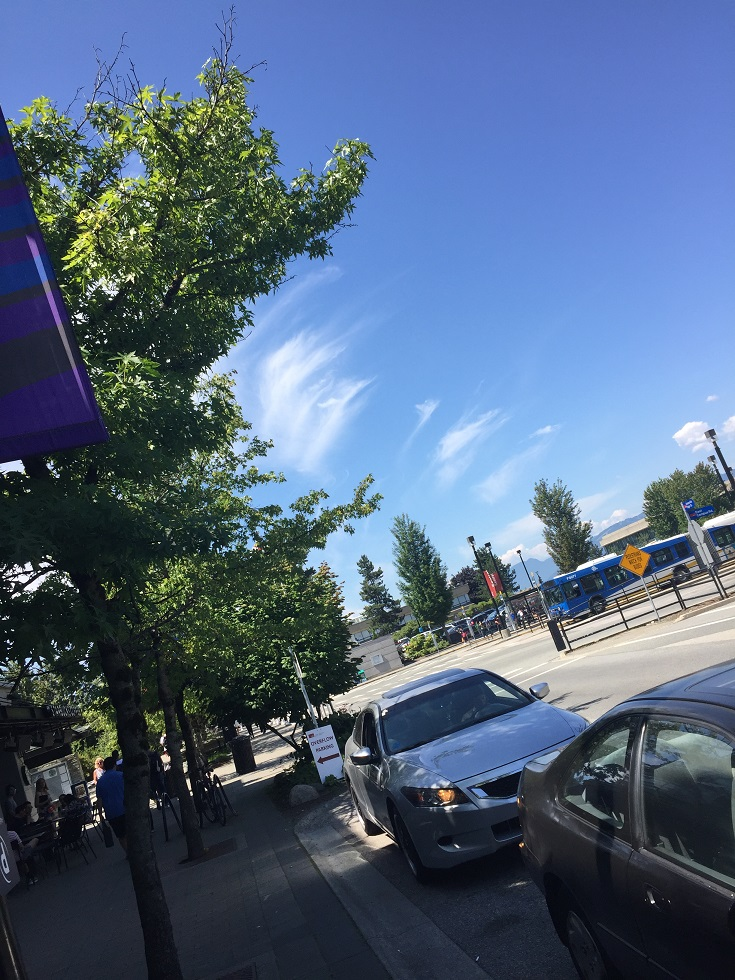
\includegraphics[scale=0.15]{results/1}
		\centering
		\caption{Image A}
	\end{subfigure}%
	\hfill
	\begin{subfigure}[h]{0.2\textwidth}
		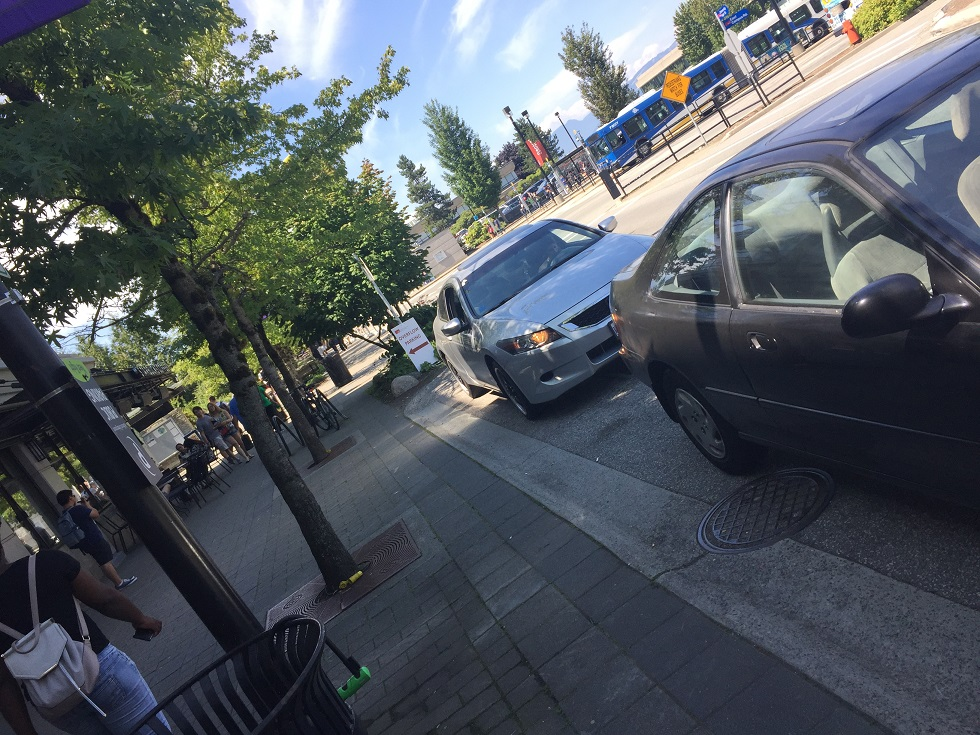
\includegraphics[scale=0.15]{results/2}
		\centering
		\caption{Image B}
	\end{subfigure}%
	\hfill
	\begin{subfigure}[h]{0.2\textwidth}
		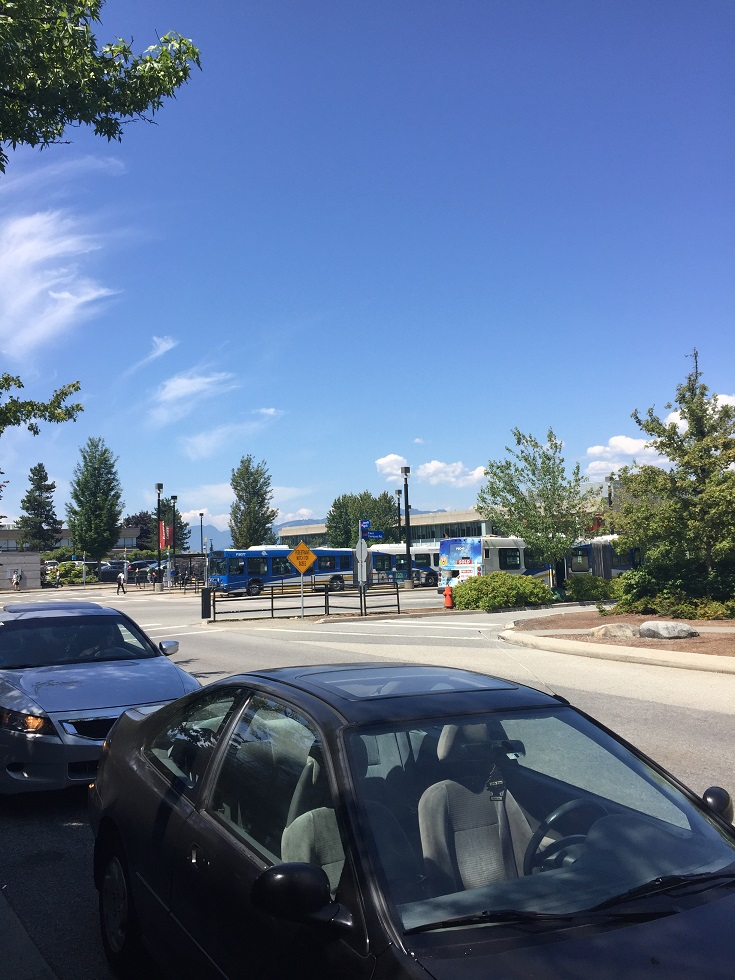
\includegraphics[scale=0.15]{results/3}
		\centering
		\caption{Image C}
	\end{subfigure}%
	\hfill
	\begin{subfigure}[h]{0.2\textwidth}
		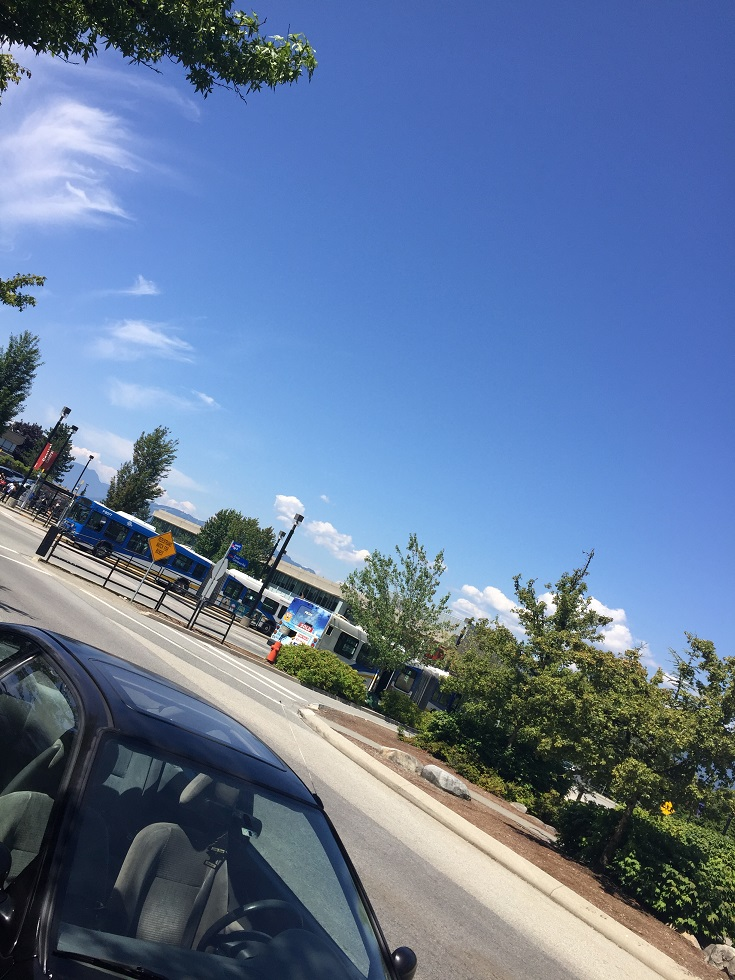
\includegraphics[scale=0.15]{results/4}
		\centering
		\caption{Image D}
	\end{subfigure}%
	\hfill
	\begin{subfigure}[h]{0.2\textwidth}
		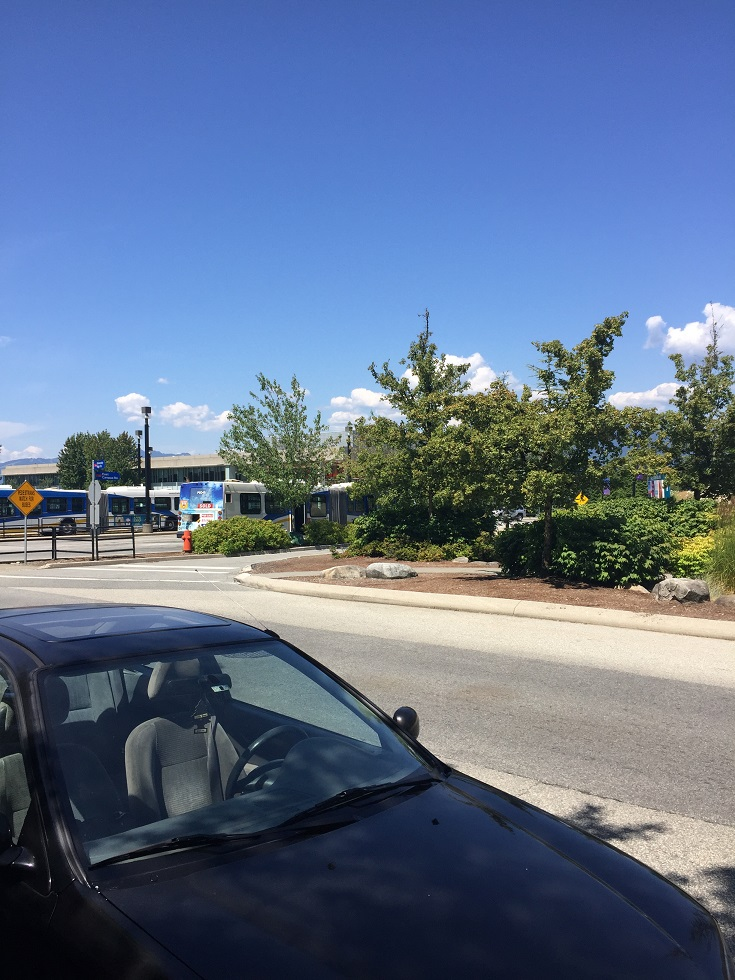
\includegraphics[scale=0.15]{results/5}
		\centering
		\caption{Image E}
	\end{subfigure}%
	\centering
\end{figure}

There are two things that break down in the aligned result. First off, there are portions of the region that are misaligned. Second and more significantly, blending does work for these images.
\vspace{30mm}

\begin{figure}[!h]
	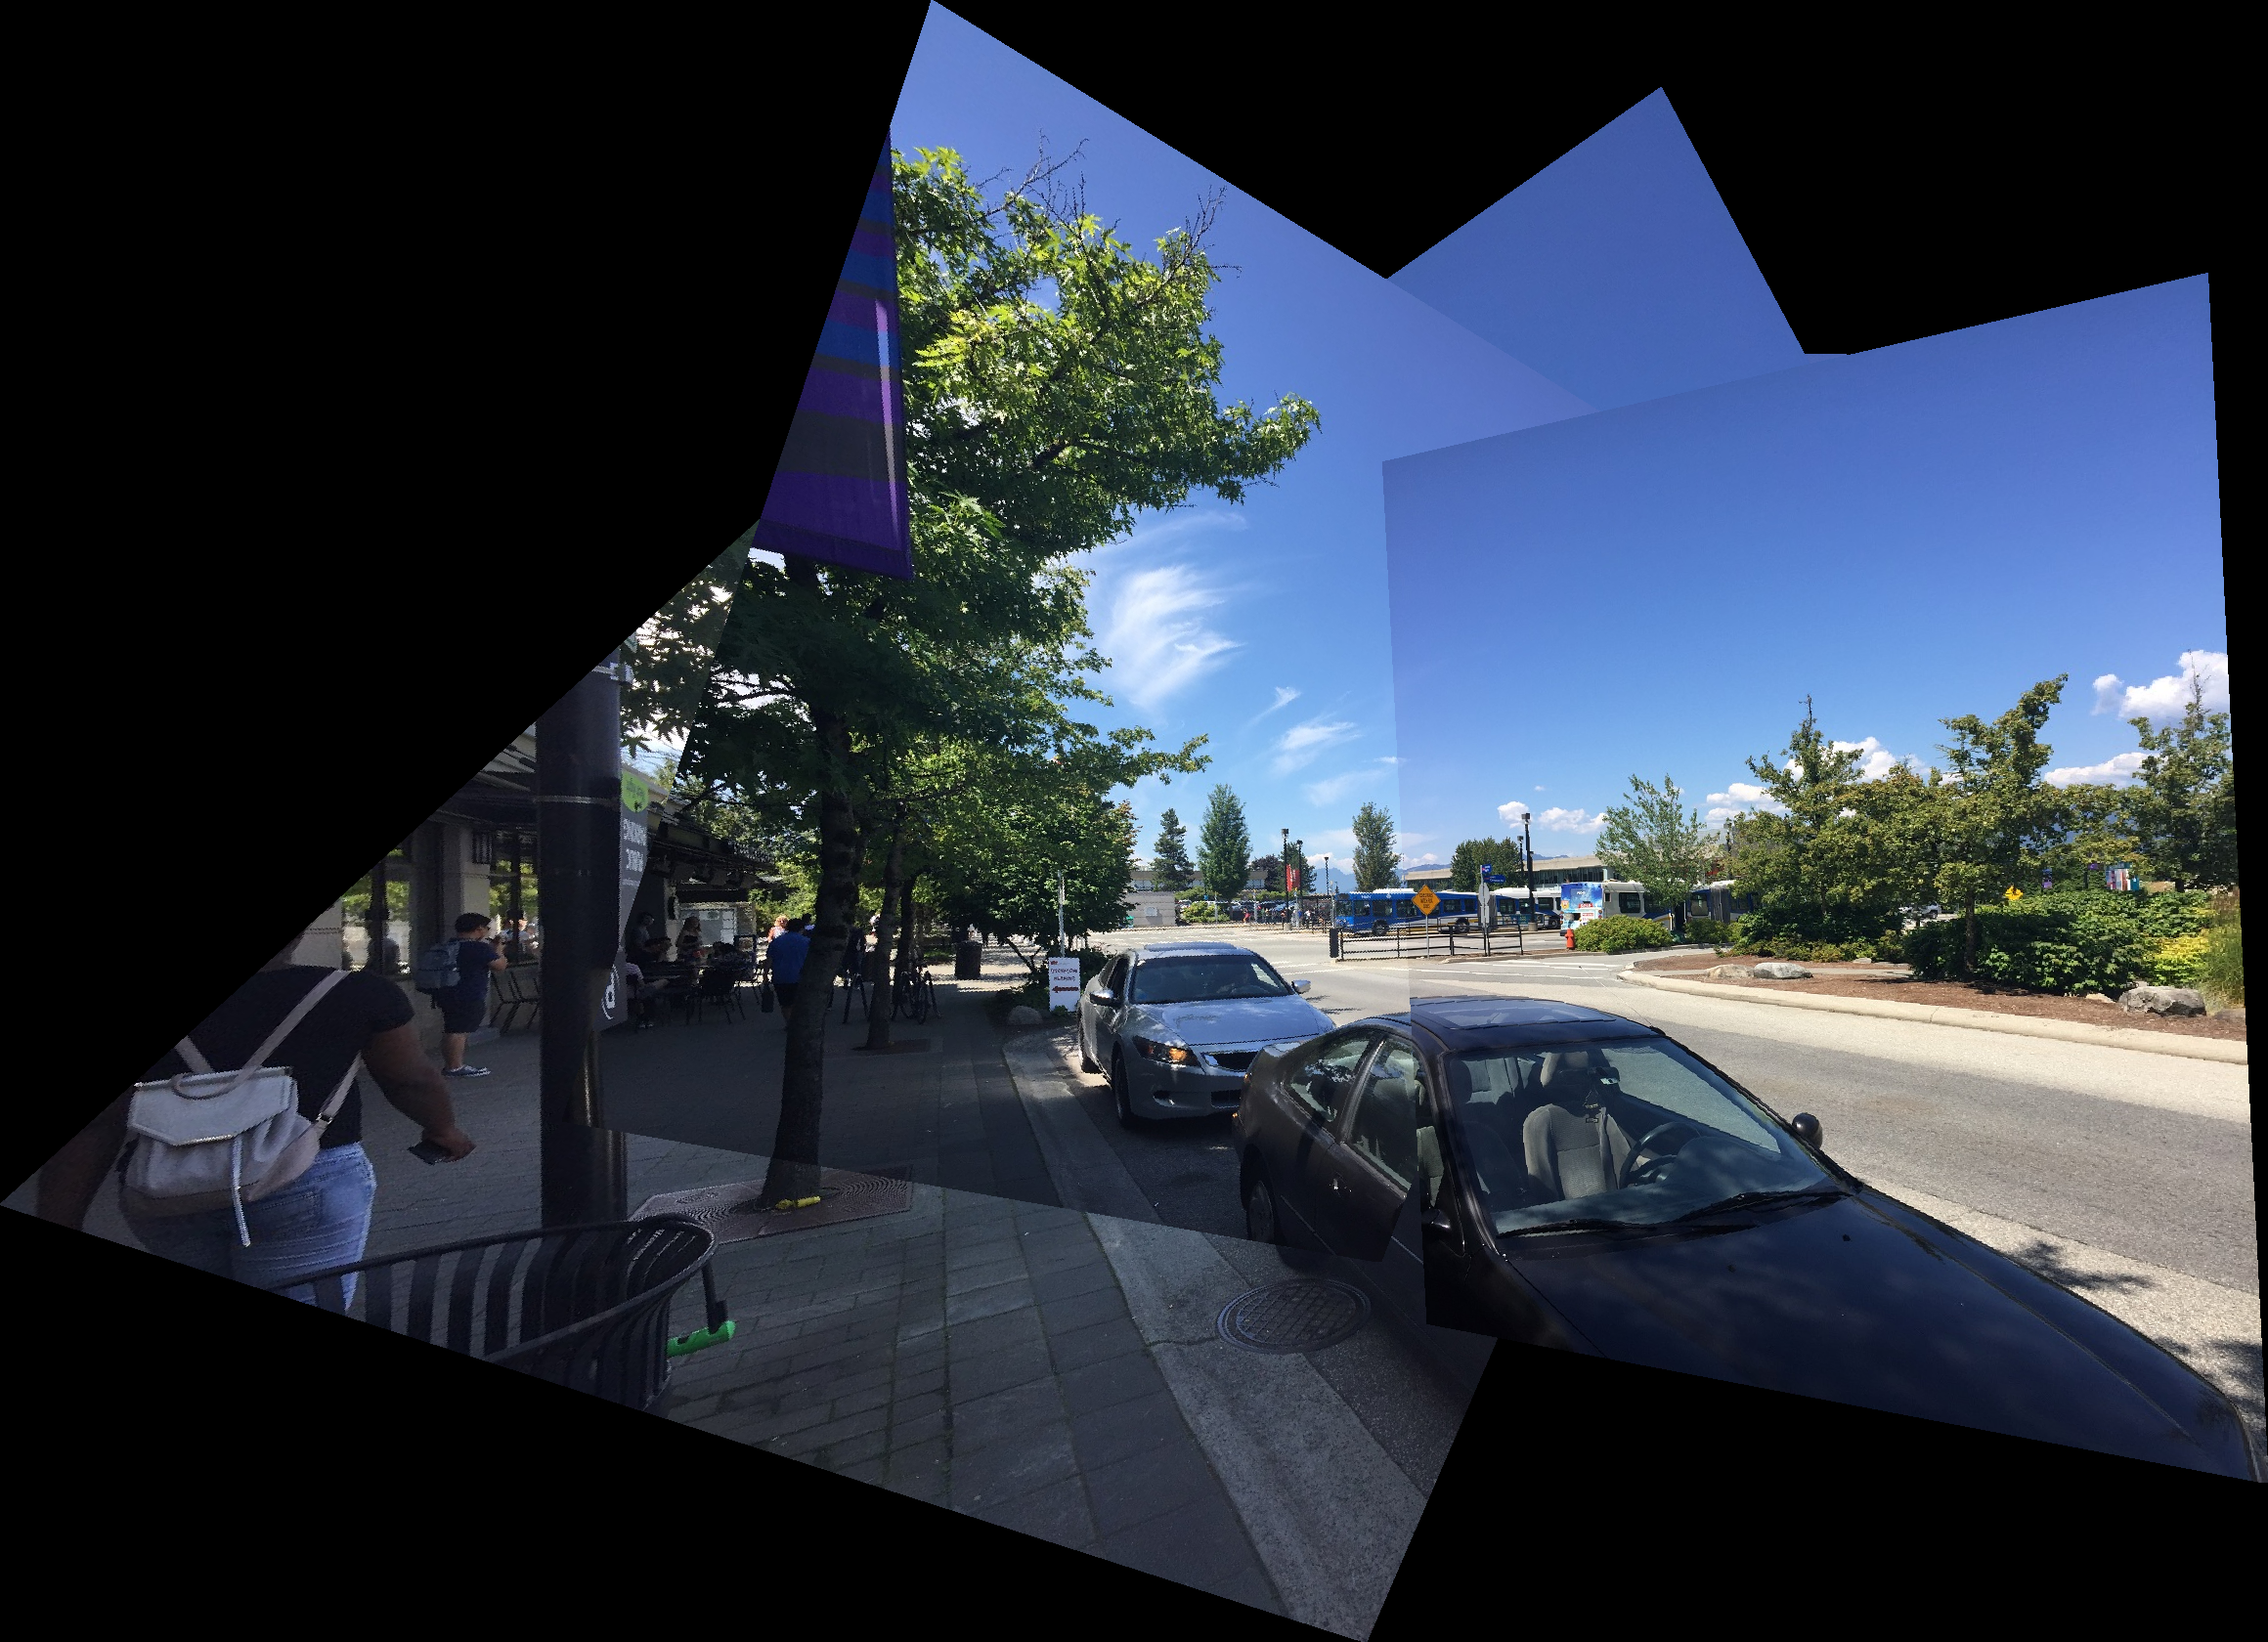
\includegraphics[scale=0.2]{results/p2_noblend/16}
	\centering
	\caption{An incorrect result: unblended}
\end{figure}
\begin{figure}[!h]
	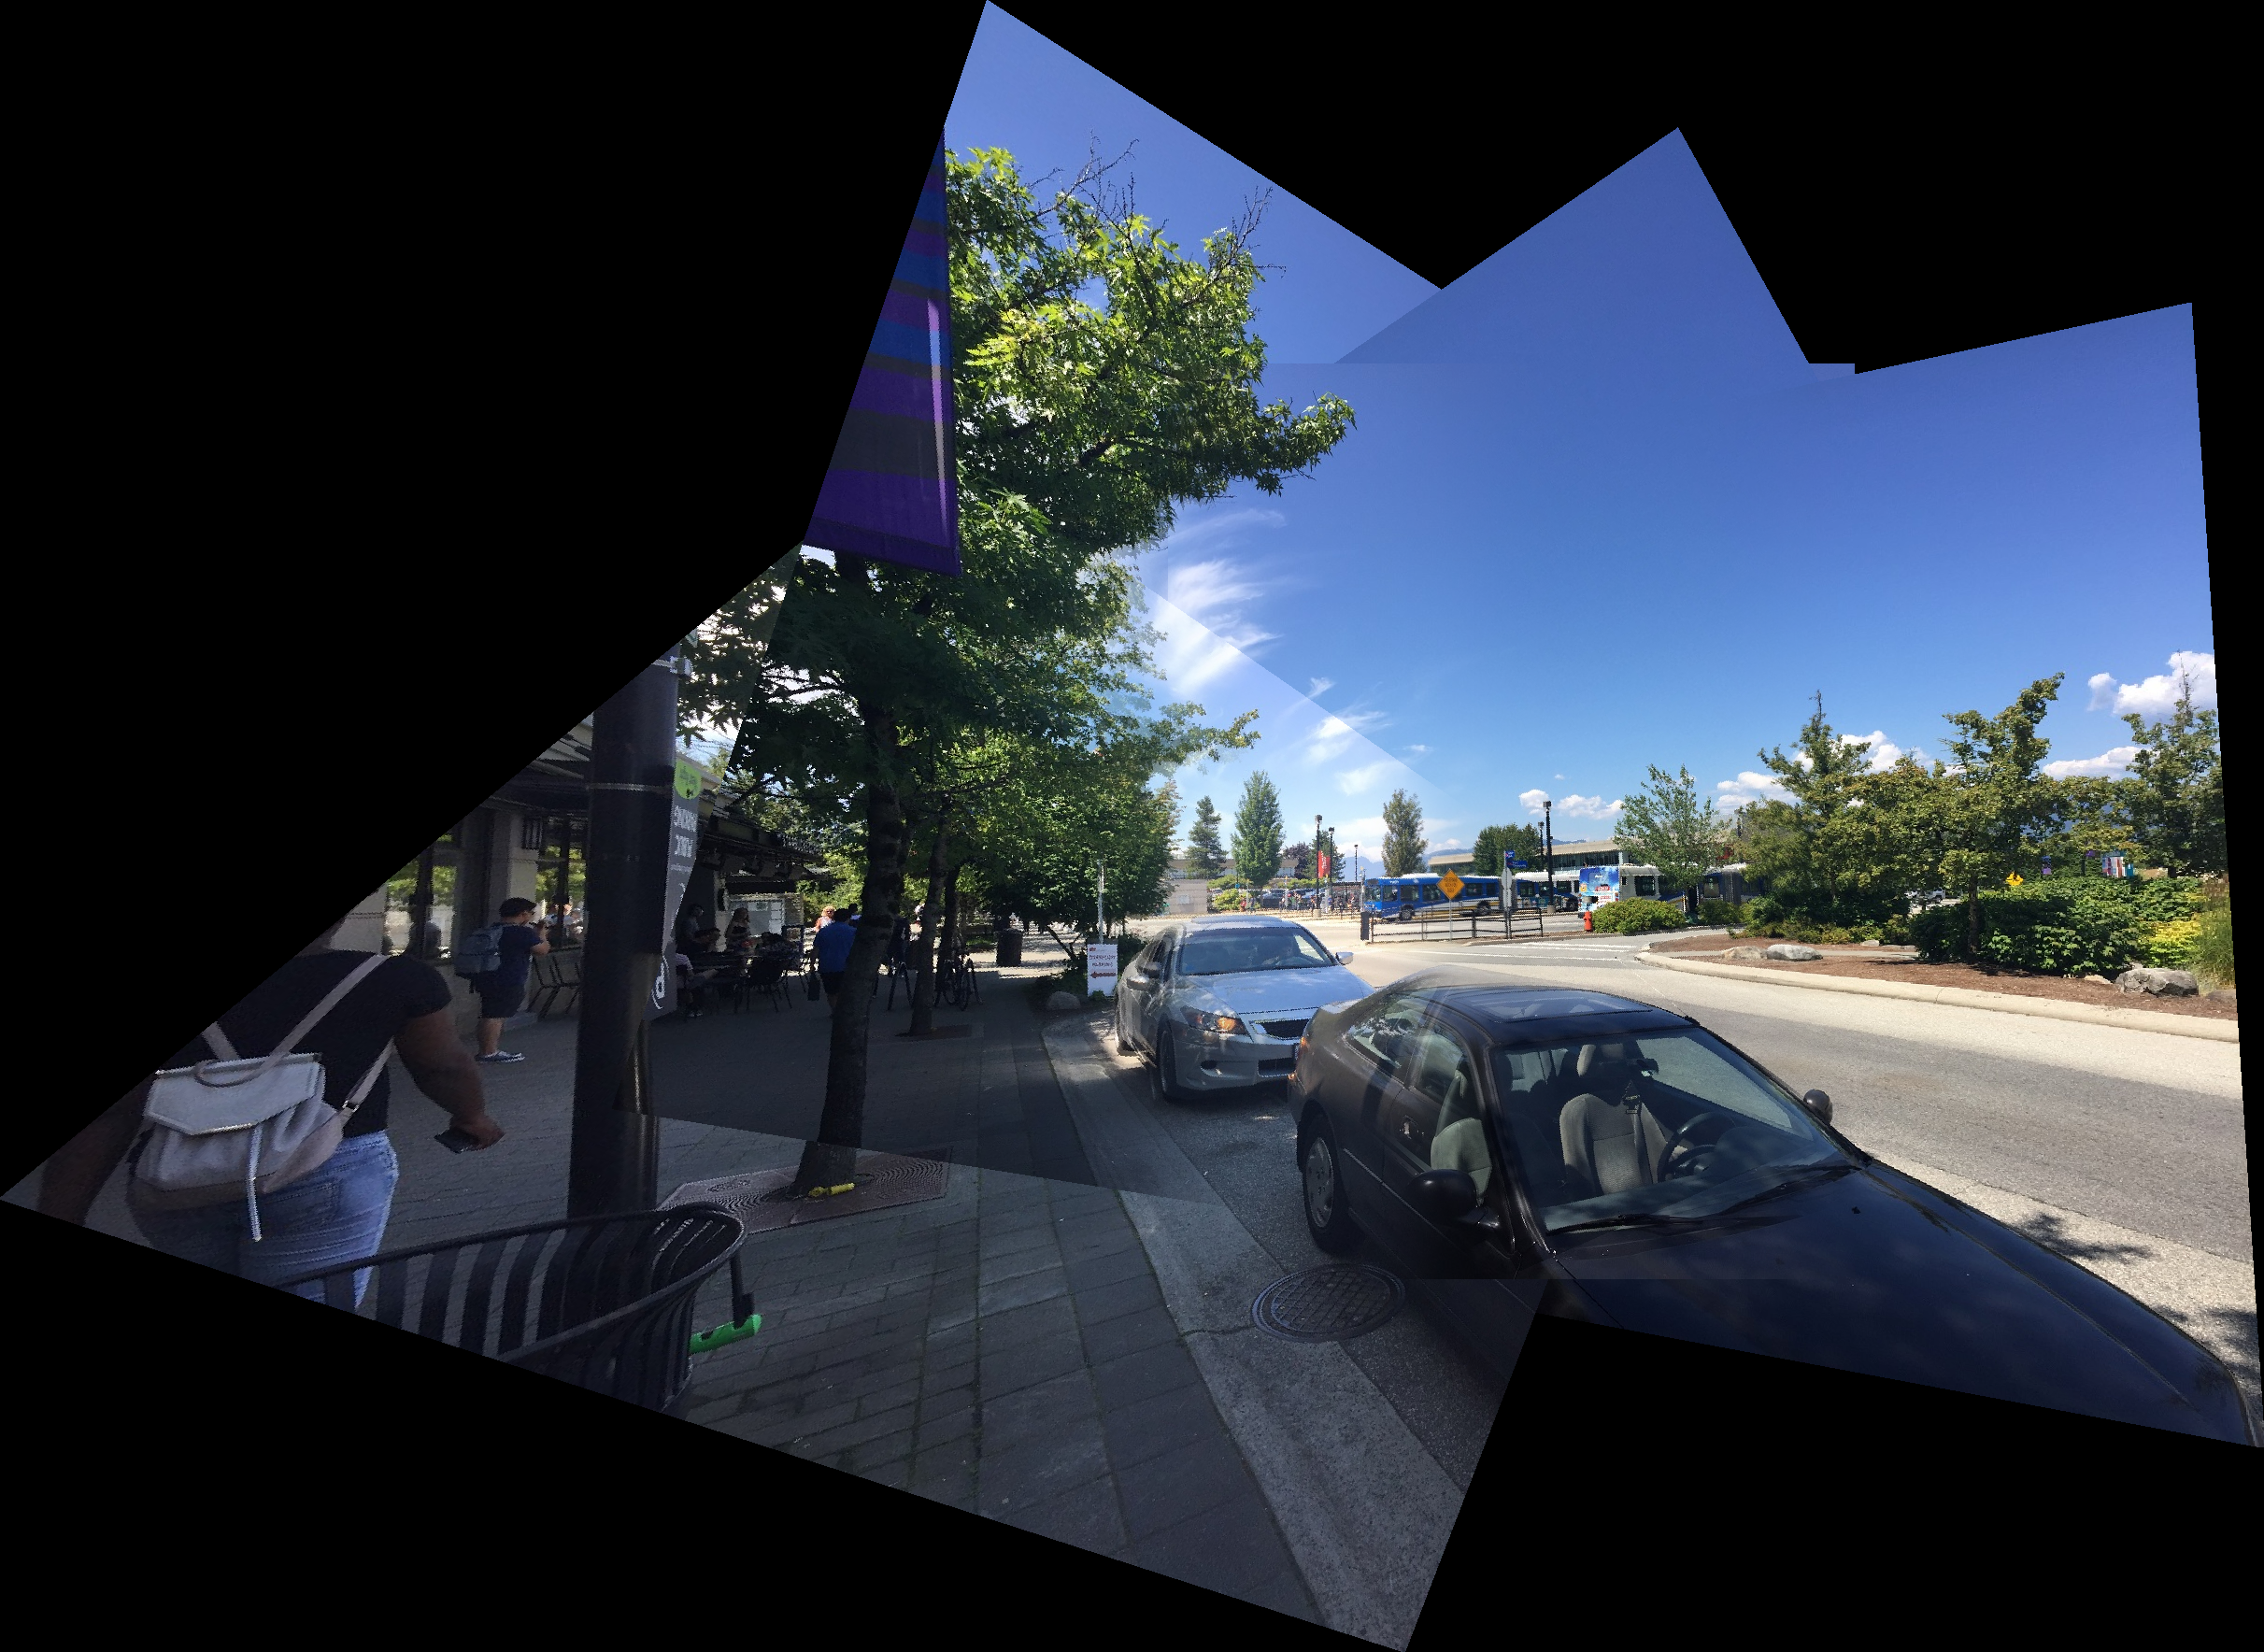
\includegraphics[scale=0.192]{results/p2_blend/16}
	\centering
	\caption{An incorrect result: blended}
\end{figure}


As we can see in the unblended version, most features of the background come together, but the gray vehicle sitting in the foreground is quite misaligned. Then, when we try to blend the result, there are some obvious issues such as 'ghosting' of the foreground vehicle and visible image seams that do not get accounted for. As far as the alignment issues go, this is more likely an issue with the input images themselves. In figure 16, the image in the left panel was taken with the camera center physically lower to the ground versus the image in the right panel. There is still a lot of correspondence between the image, but the nature of RANSAC and how it finds inliers ultimately forces alignment of either the foreground or background. When counting inliers, if the background is aligned, then foreground inliers will not be, and if features of the foreground are aligned, then inliers in the background will not be. In this case, RANSAC ultimately found a stronger correspondence in the background features, and after projection, we see how most of the background is well aligned, but the foreground is not. And as soon as this happens once, any images to follow will also likely be misaligned.

\begin{figure}[!h]
	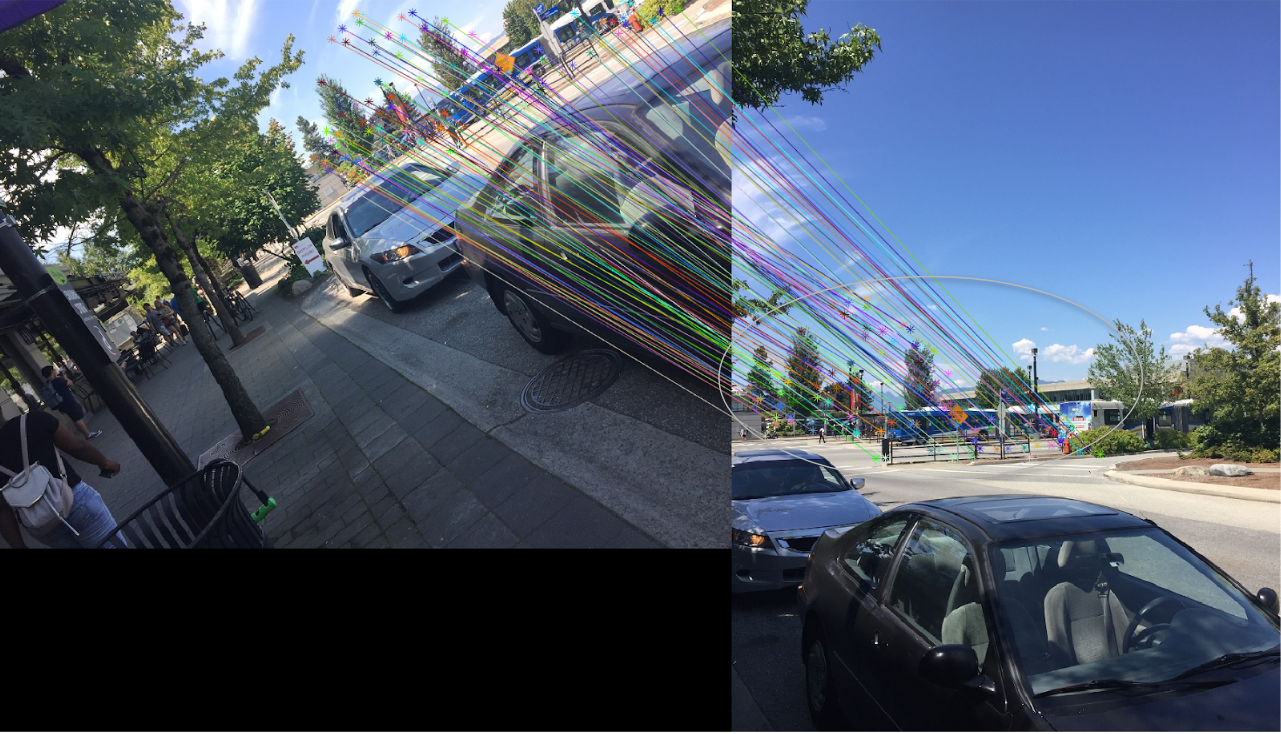
\includegraphics[scale=0.5]{results/issue1}
	\centering
	\caption{The inliers produced from RANSAC matching the two images }
\end{figure}
\begin{figure}[!h]
	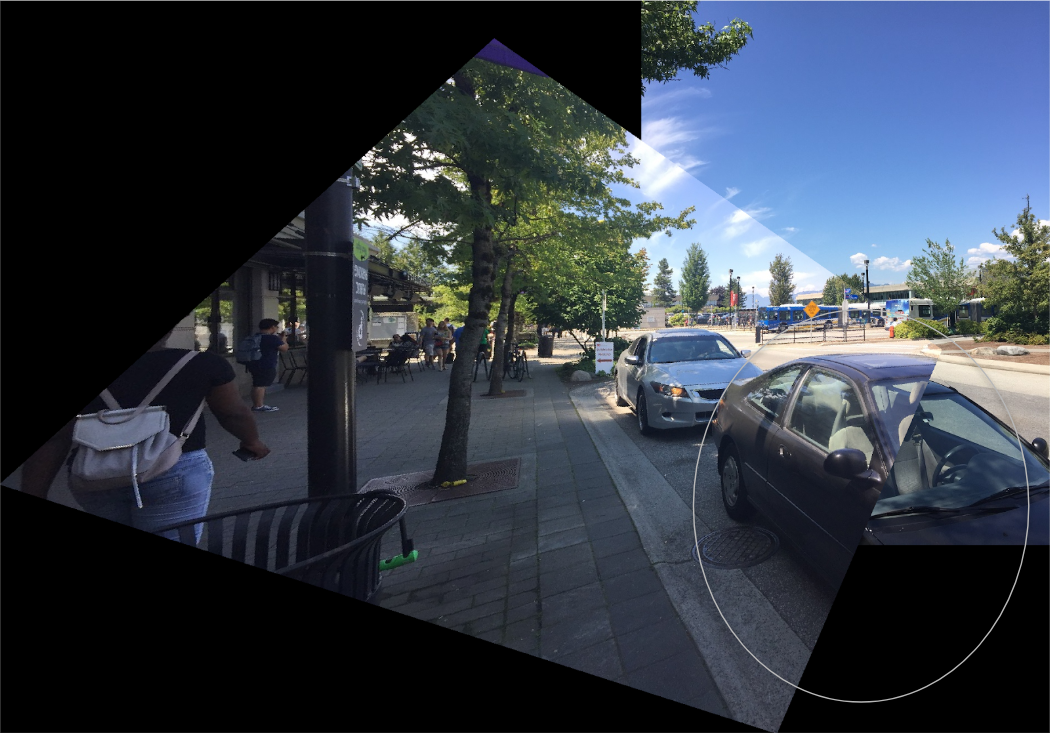
\includegraphics[scale=0.6]{results/issue2}
	\centering
	\caption{The resulting alignment with the foreground very misaligned}
\end{figure}
\vspace{10mm}

There is one more observation to make regarding feature matching of multiple images. In all of the examples so far, we are projecting images onto already warped images. For example, consider the following images A, B, and C being aligned by method 1, which is the same as what we have been doing so far:

\begin{figure}[h]
	\begin{subfigure}[h]{0.5\textwidth}
		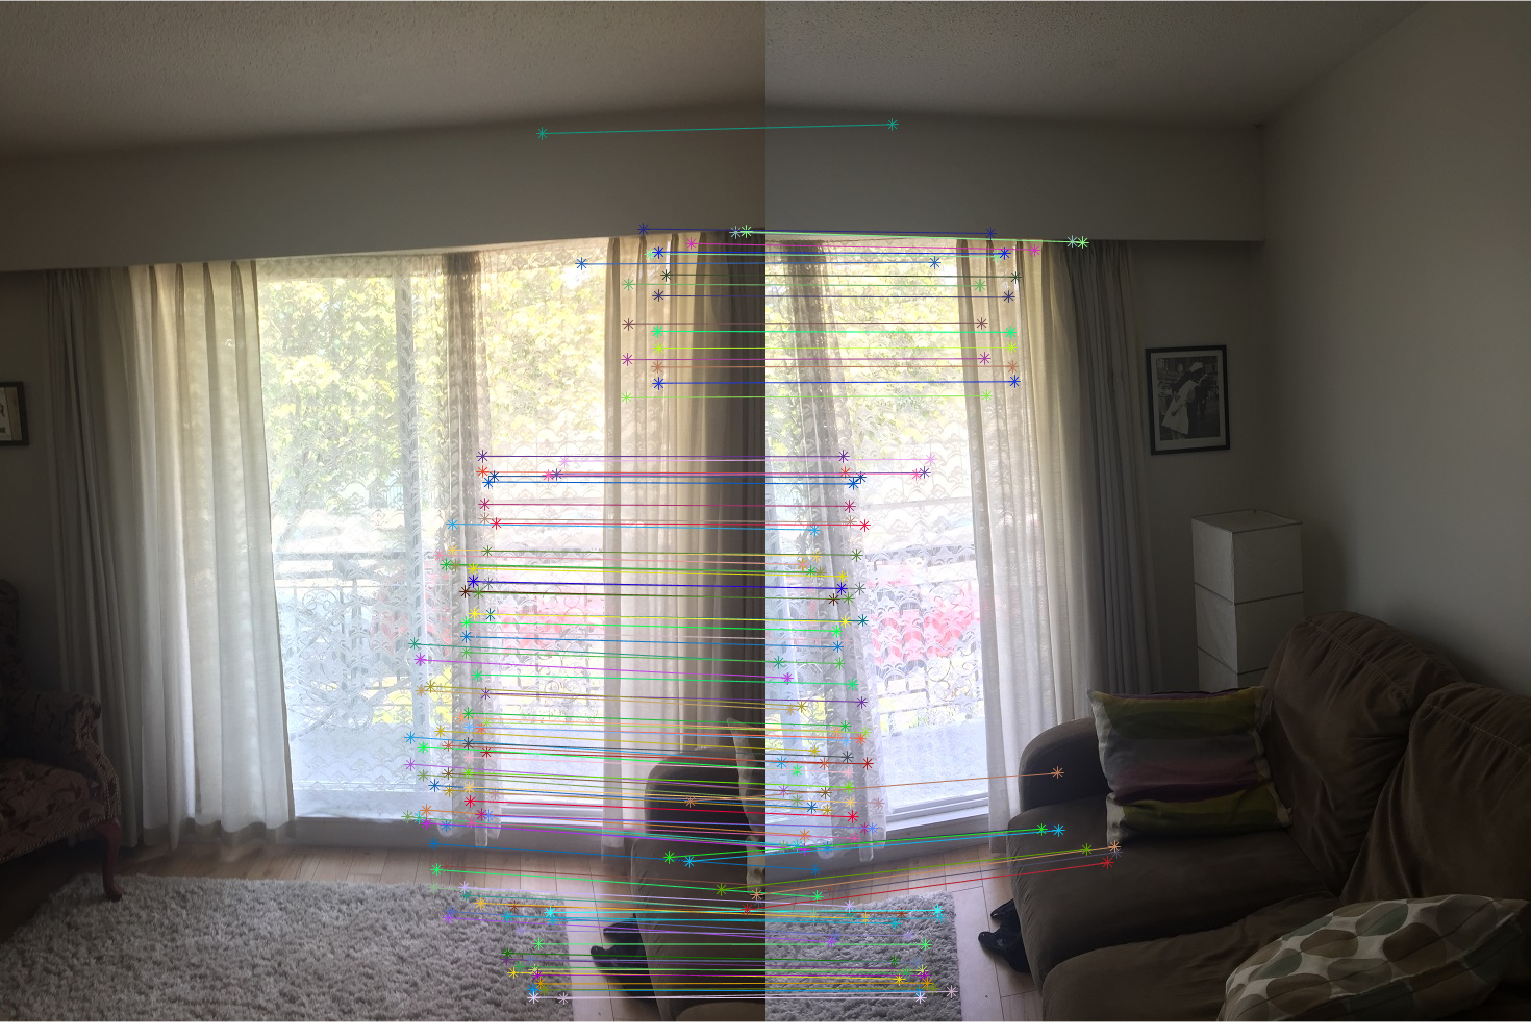
\includegraphics[scale=0.35]{results/SIFT_indifference/method1/7}
		\centering
		\caption{Left: Image A, Right: Image B}
	\end{subfigure}%
	\hfill
	\begin{subfigure}[h]{0.5\textwidth}
		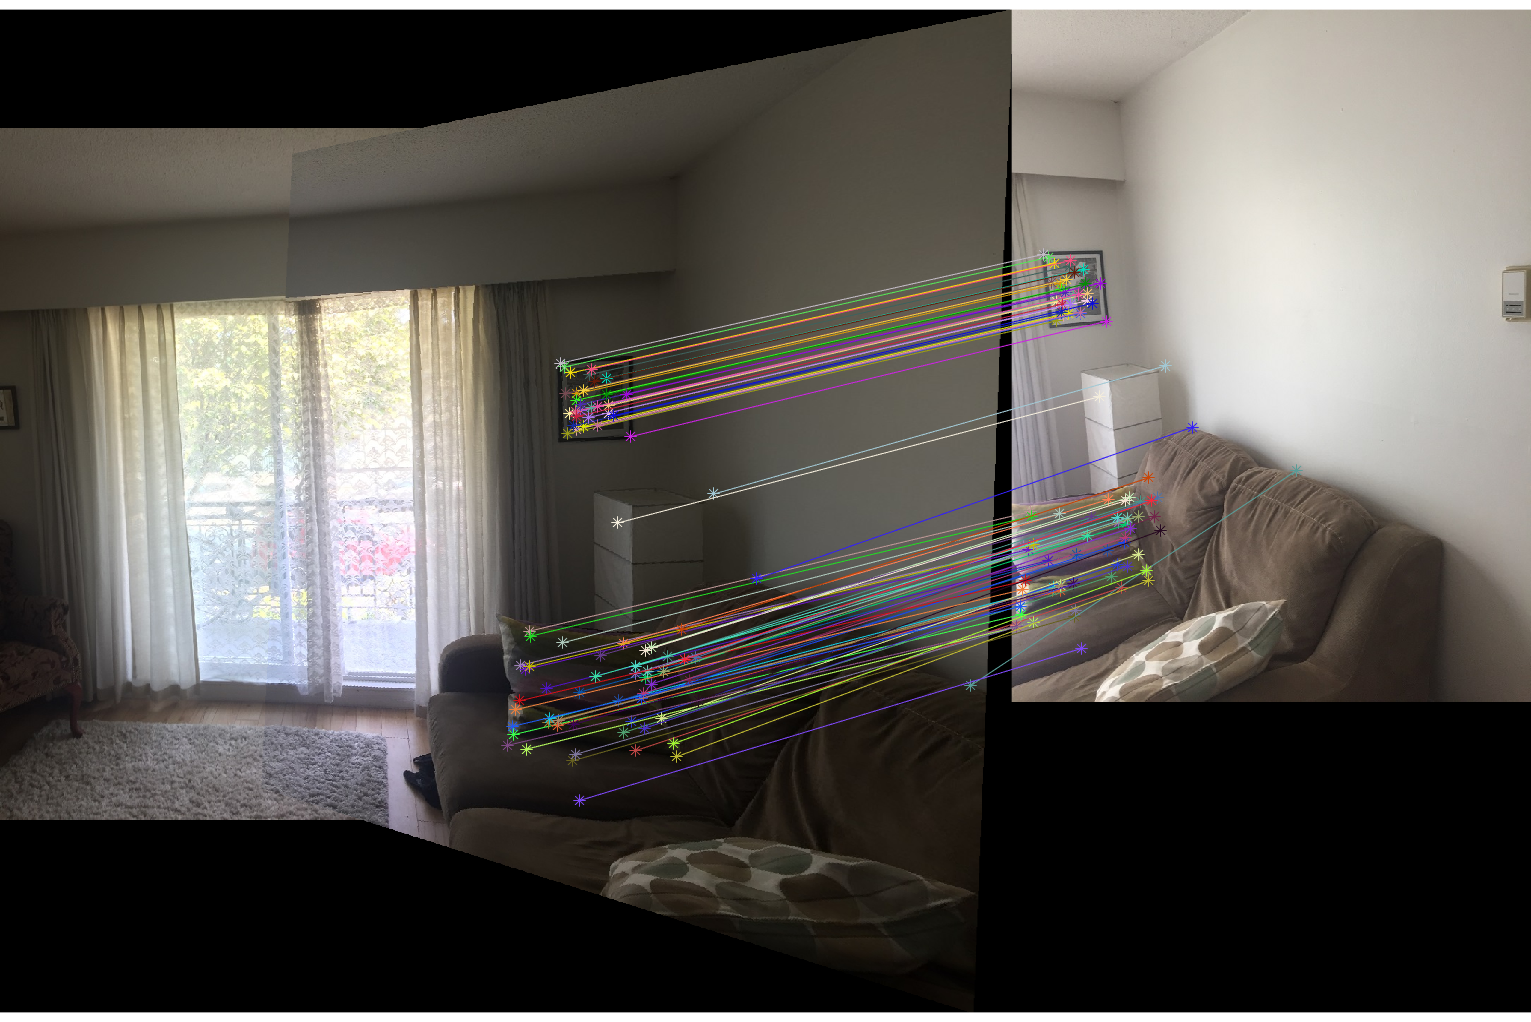
\includegraphics[scale=0.35]{results/SIFT_indifference/method1/15}
		\centering
		\caption{Left: Image B projected onto A, Right: Image C}
	\end{subfigure}%
	\centering
	\caption{Inliers found by RANSAC during aligning of images A, B, C using method 1}
\end{figure}

The issue here is with image C, where we more or less trying to match features with image B. But image B has already been warped, and so we are trying to match features from a warped image to an unwarped one. It seems that this could potentially pose as an issue, but if we knew that image C was essentially to be projected onto image B, and that image B was to be projected onto image A, then perhaps there's a better way to go about aligning C.

As an alternative, if we knew the homography $H_1$ for projecting B onto A and $H_2$ for projecting C onto (the unwarped) B, then we could project C onto A by the homography $H_1H_2$. This way, we wouldn't have to worry about matching features to warped images.

\begin{figure}[h]
	\begin{subfigure}[h]{0.5\textwidth}
		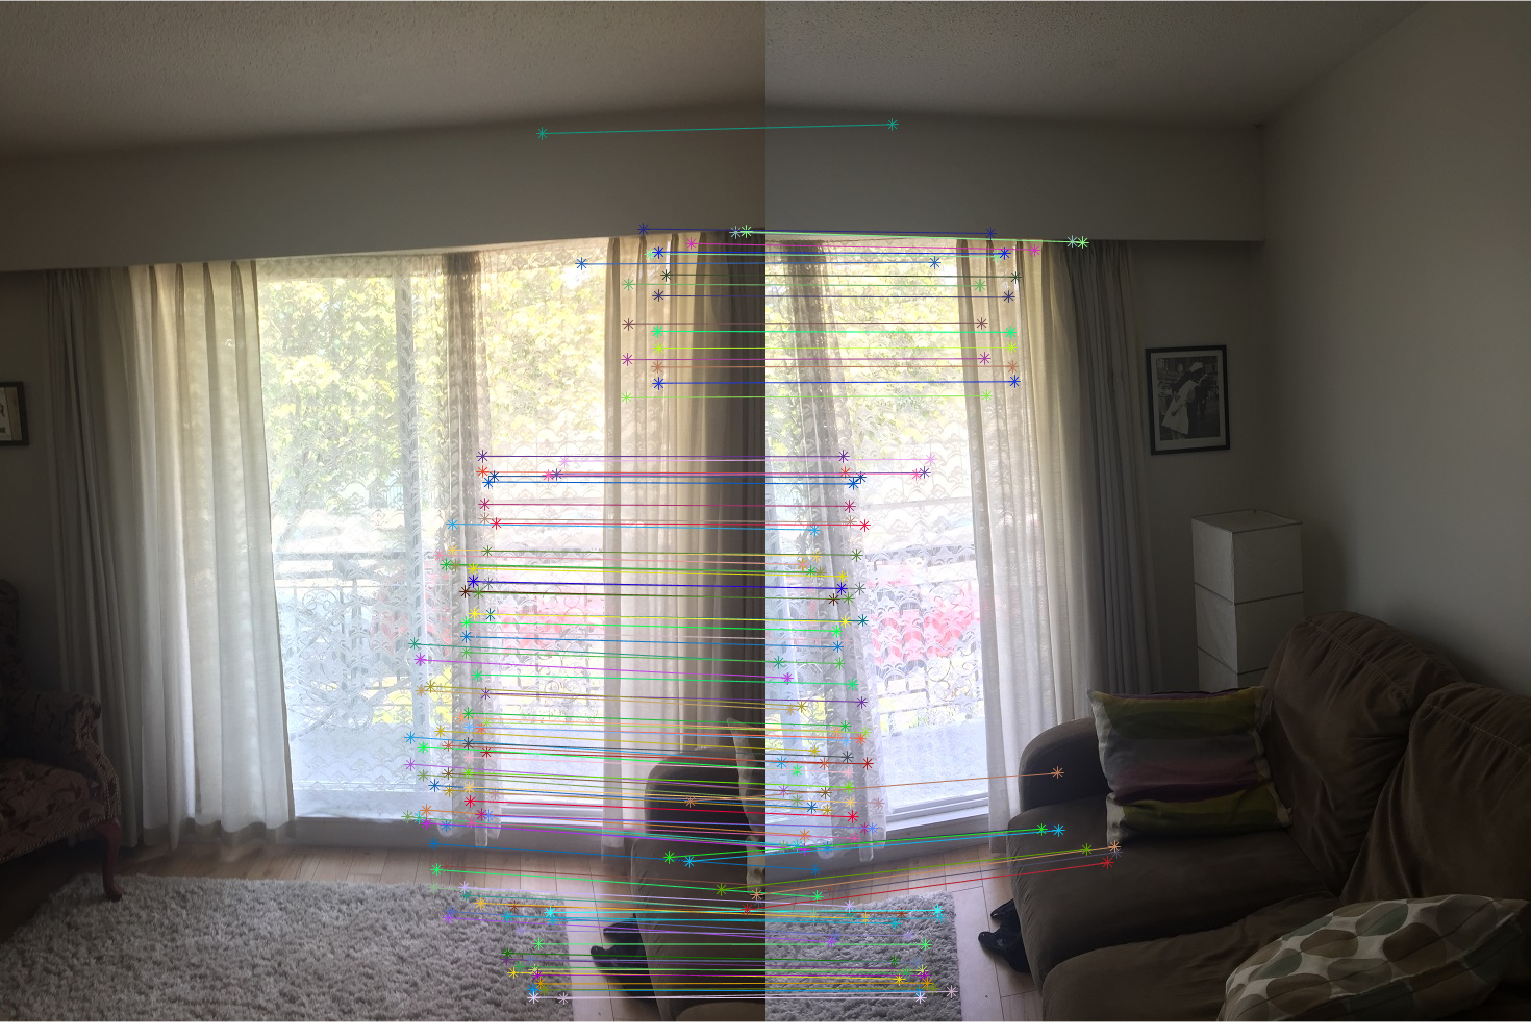
\includegraphics[scale=0.35]{results/SIFT_indifference/method1/7}
		\centering
		\caption{Finding $H_1$}
	\end{subfigure}%
	\hfill
	\begin{subfigure}[h]{0.5\textwidth}
		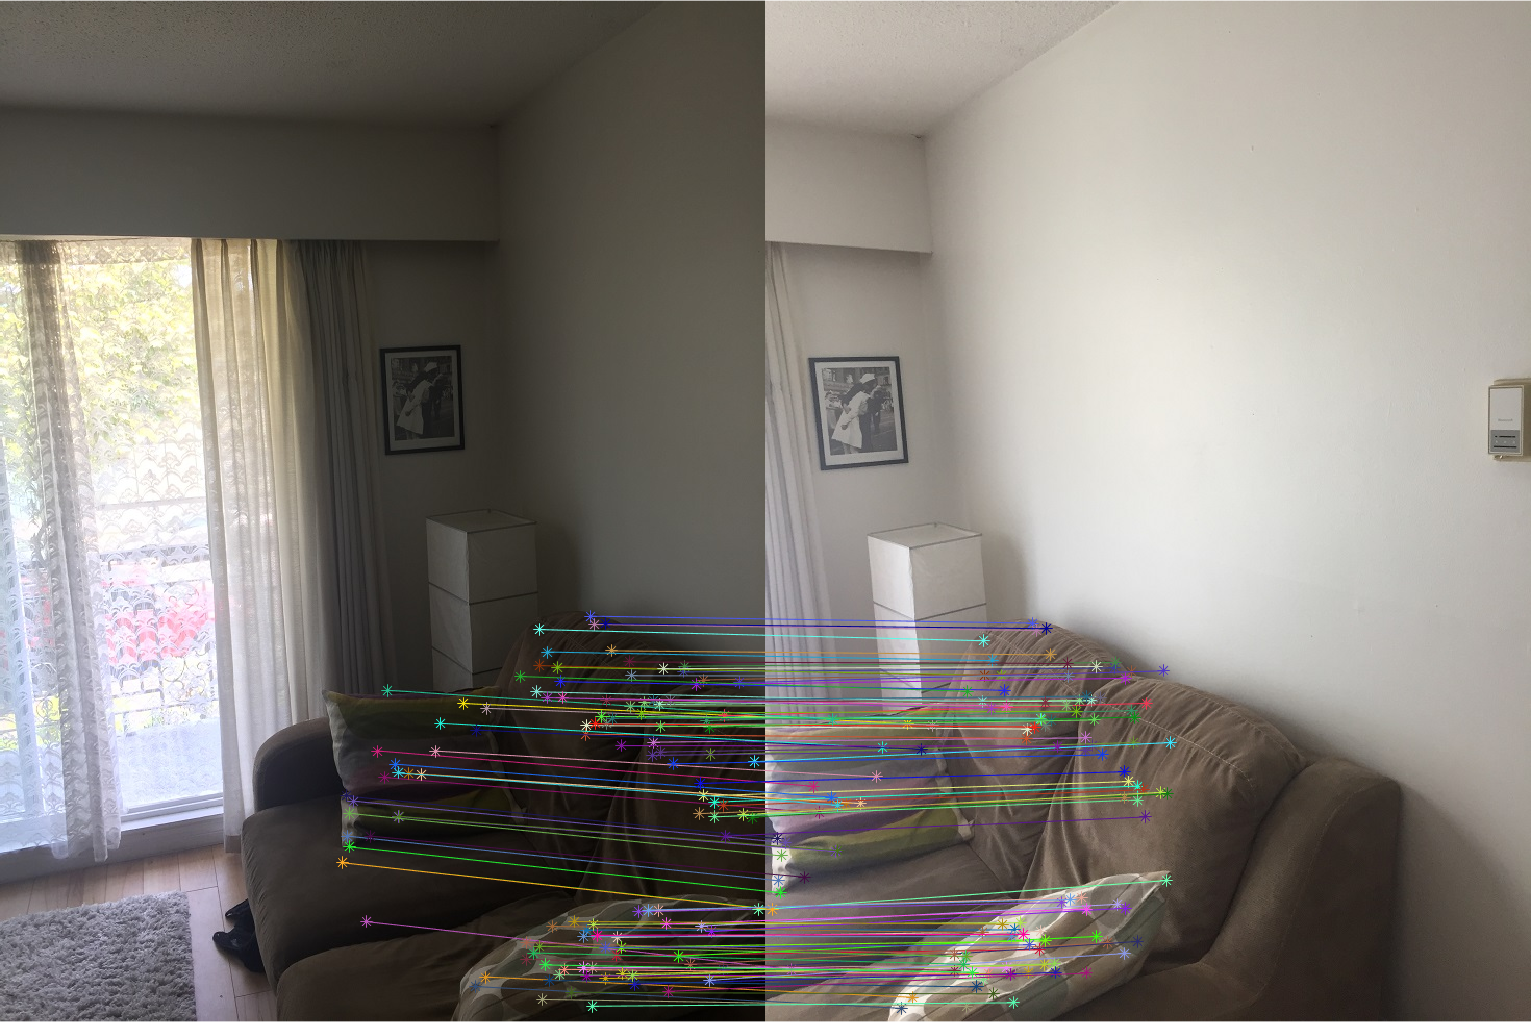
\includegraphics[scale=0.35]{results/SIFT_indifference/method2/3}
		\centering
		\caption{Finding $H_2$ using the unwarped image B as reference}
	\end{subfigure}%
	\centering
	\caption{Inliers found by RANSAC during aligning of images A, B, C using method 2}
\end{figure}

However, in all of the comparisons performed using both methods, no significant improvement could be found using one method over the other. The following figures depict the results using the two methods, and it seems that up to expected variations in the approximated homography, they are identical in terms of quality.

\vspace{100mm}

\begin{figure}[!h]
	\begin{subfigure}[!h]{0.5\textwidth}
		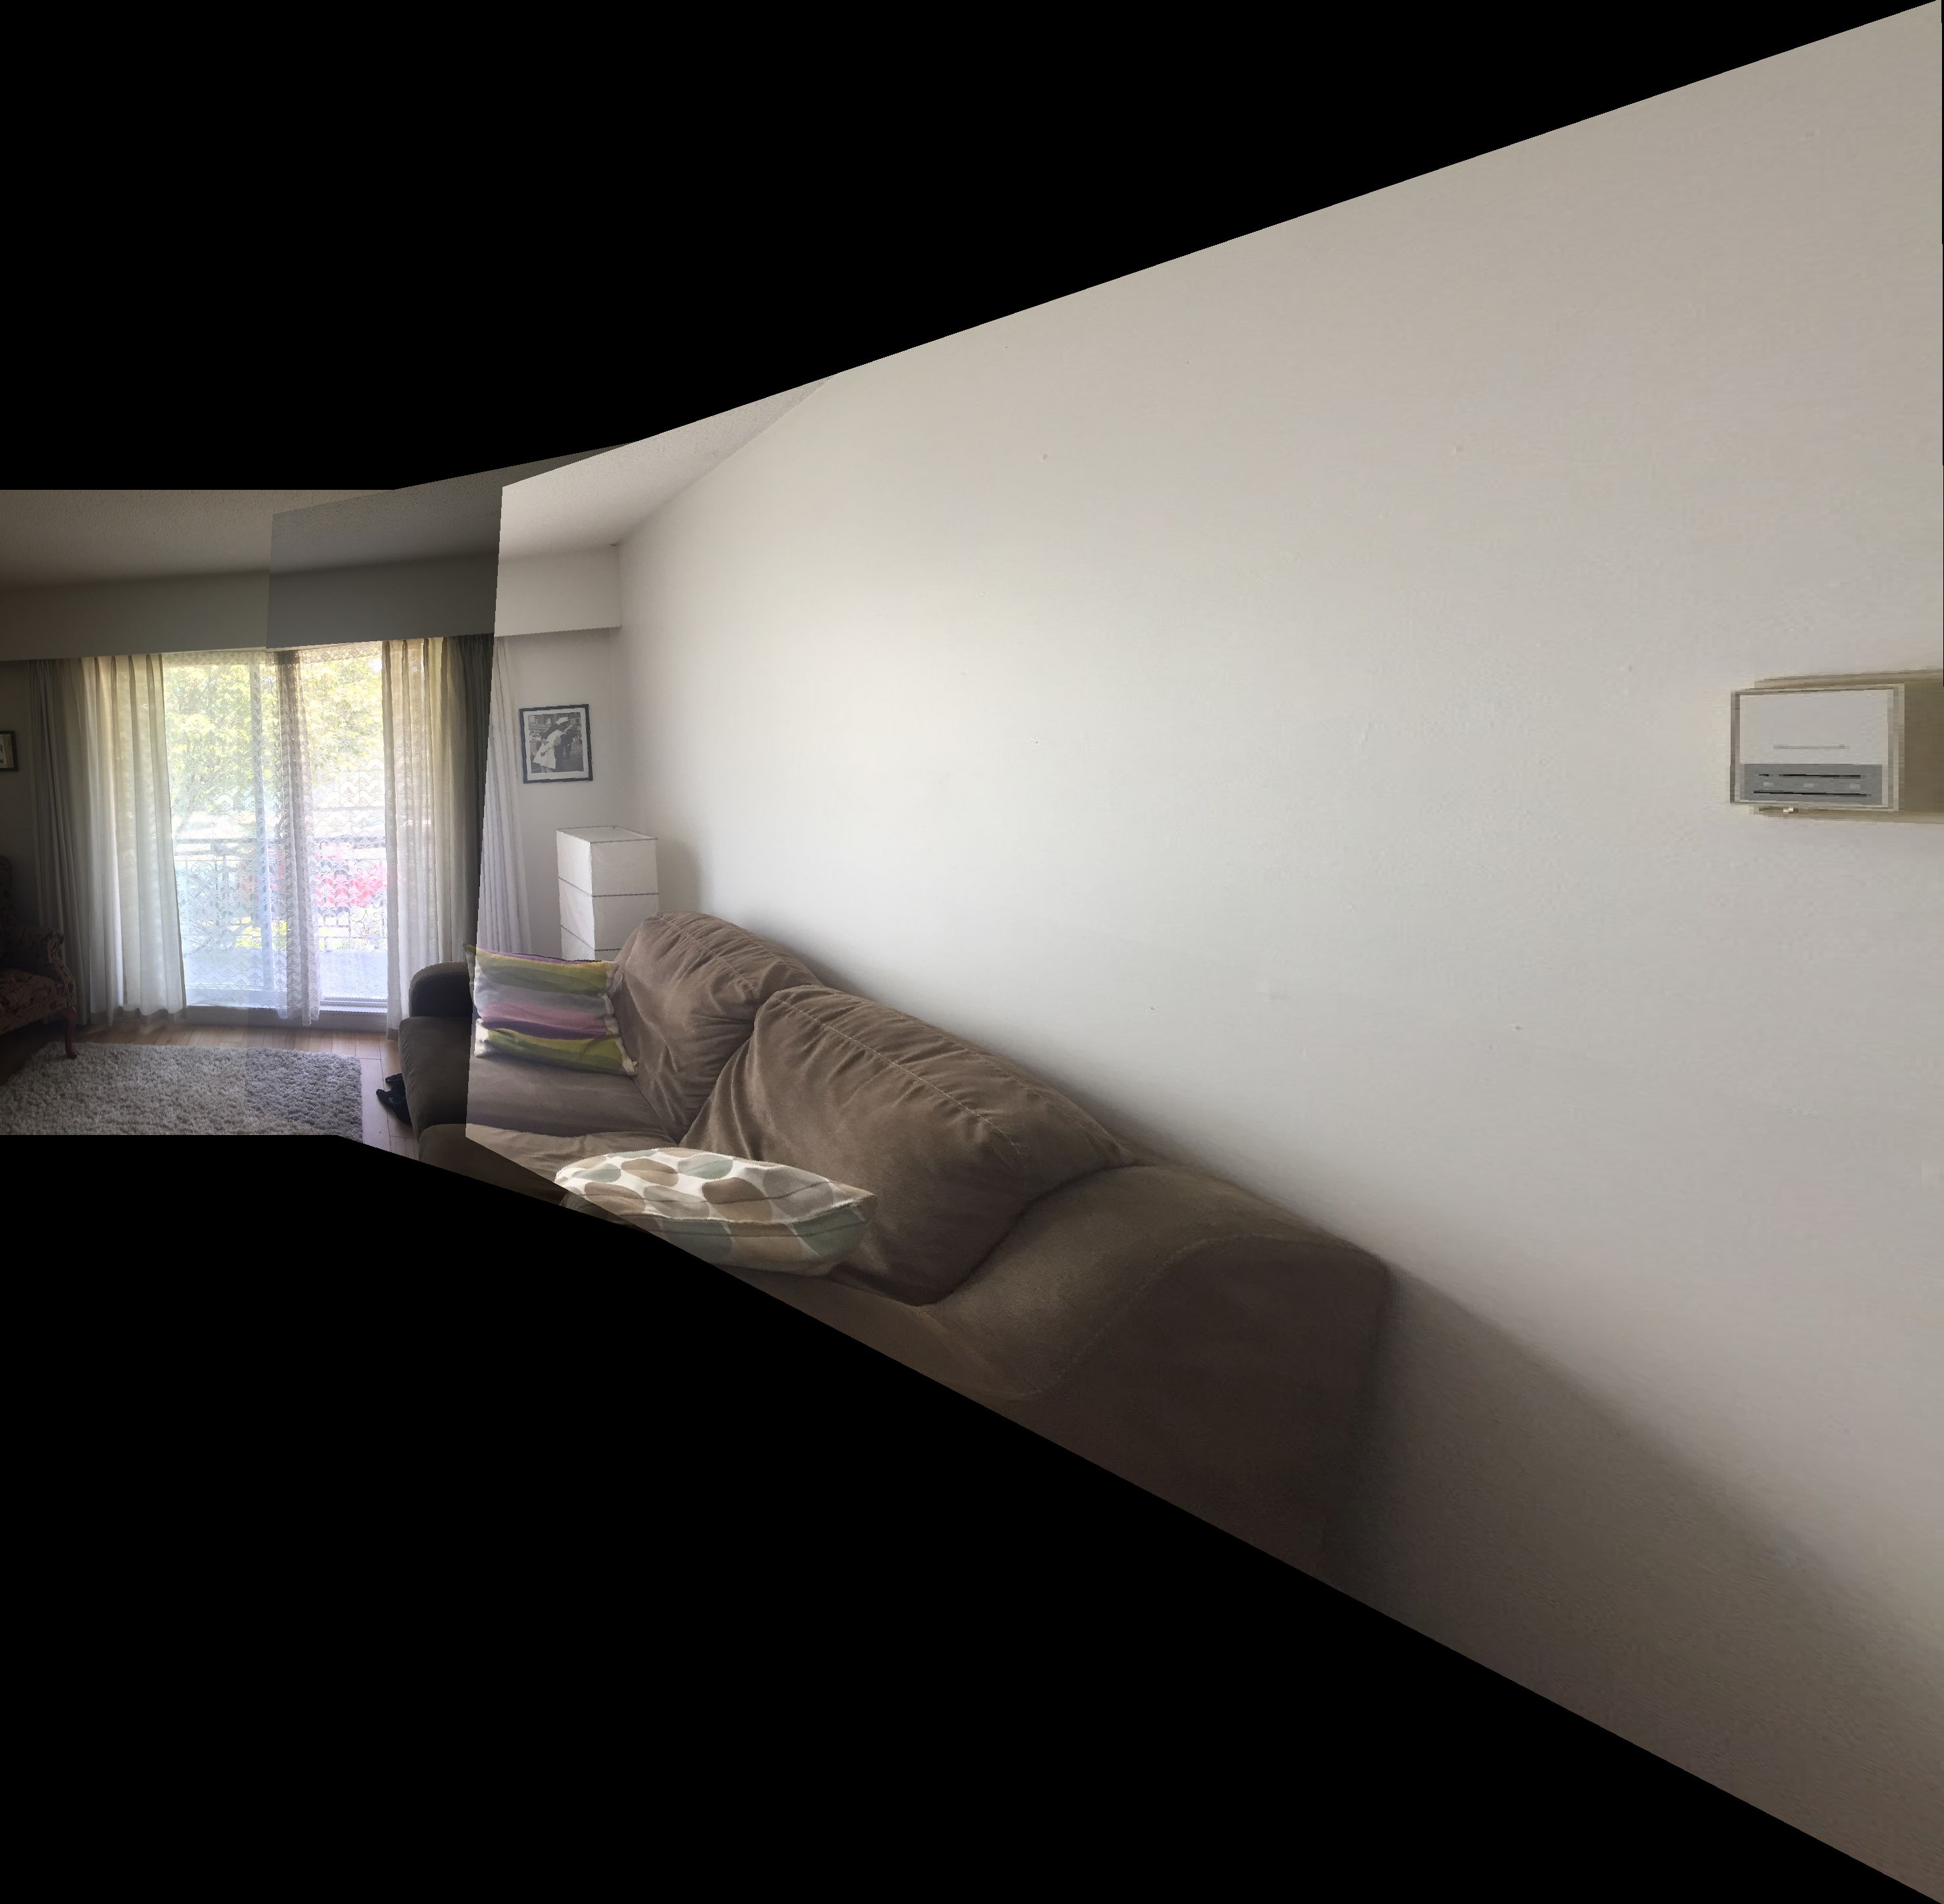
\includegraphics[scale=0.091]{results/SIFT_indifference/method1/16}
		\centering
		\caption{Method 1}
	\end{subfigure}%
	\hfill
	\begin{subfigure}[!h]{0.5\textwidth}
		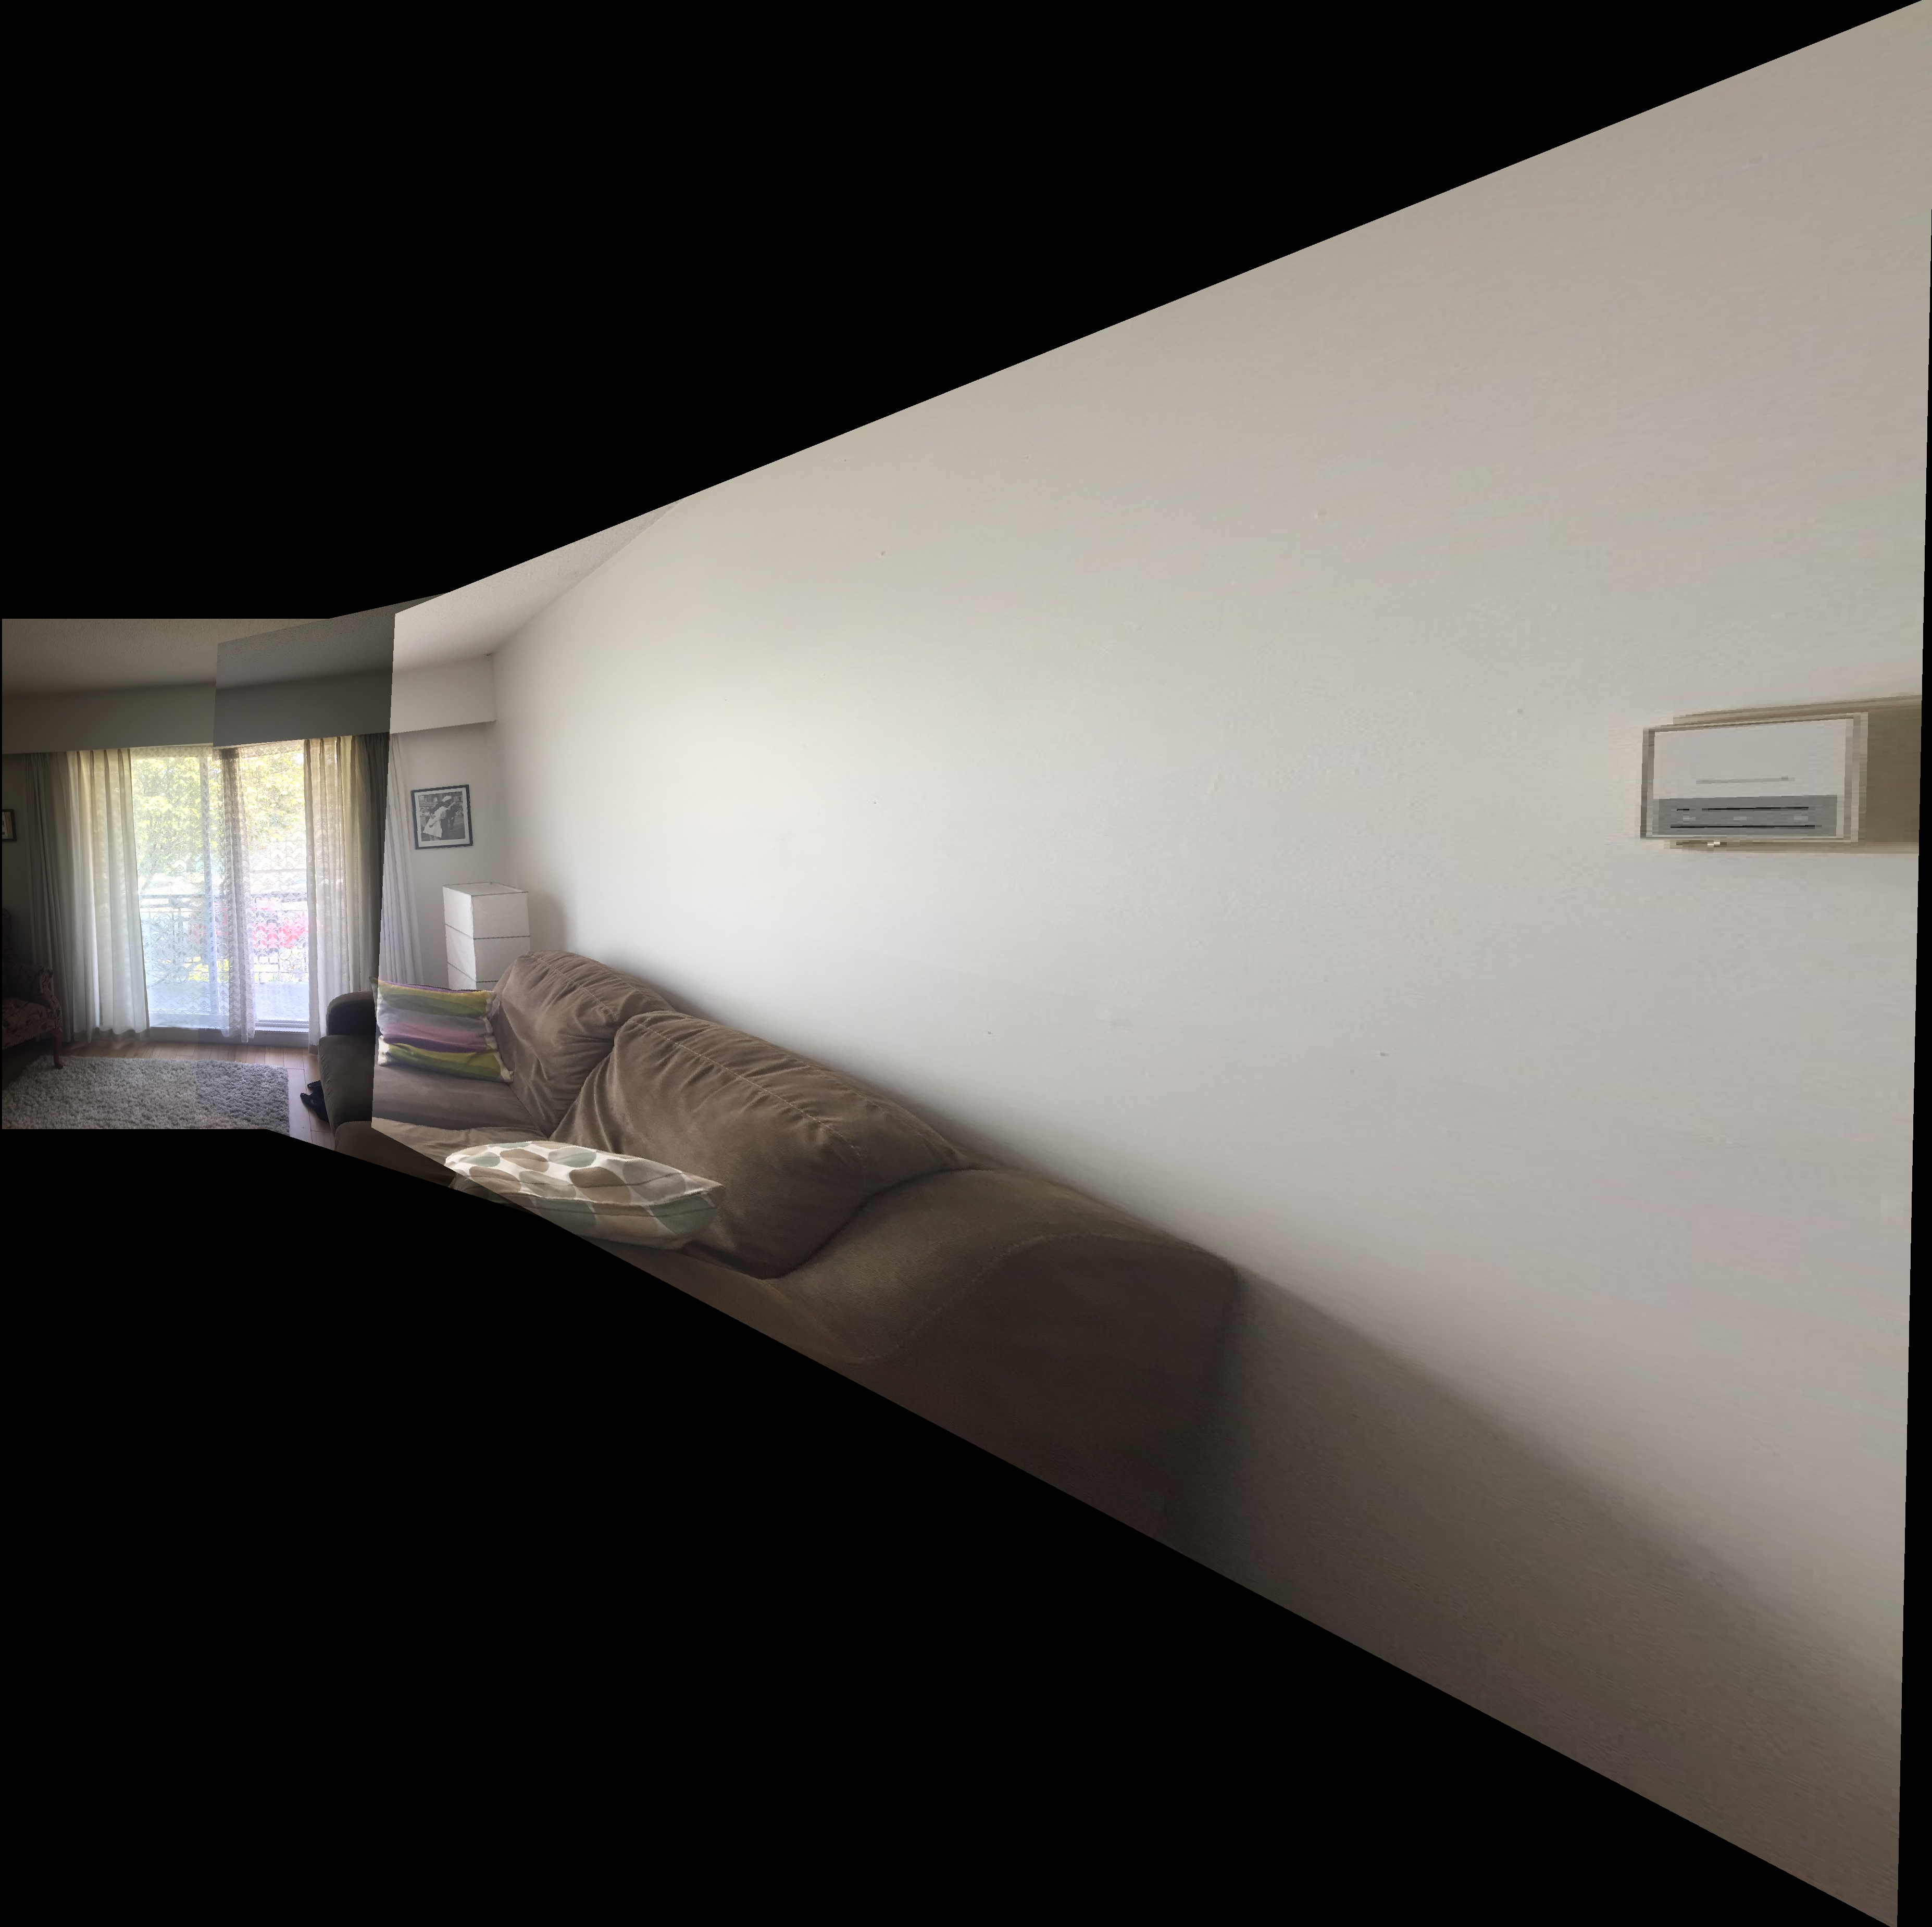
\includegraphics[scale=0.095]{results/SIFT_indifference/method2/8}
		\centering
		\caption{Method 2}
	\end{subfigure}%
	\centering
	\caption{Comparing method 1 and method 2}
\end{figure}

As a final remark, one of the goals for this project was to have it so that this process was essentially automated, in the sense that no parameterization needed to be adjusted between sets of images. After the overall 'best' settings were found, this was more or less achieved. For images that fit the intended conditions such as aligning into a horizontal orientation, the default settings usually produced good results.

\vspace{5mm}
\textbf{3) Additional Results}
\vspace{3mm}

Following are some additional results which turned out well.

\begin{figure}[!h]
	\includegraphics[scale=0.17]{results/p5_noblend/16}
	\centering
	\caption{Unblended version}
\end{figure}
\vspace{300mm}
\begin{figure}[!h]
	\includegraphics[scale=0.17]{results/p5_blended/16}
	\centering
	\caption{Blended version}
\end{figure}
\begin{figure}[!h]
	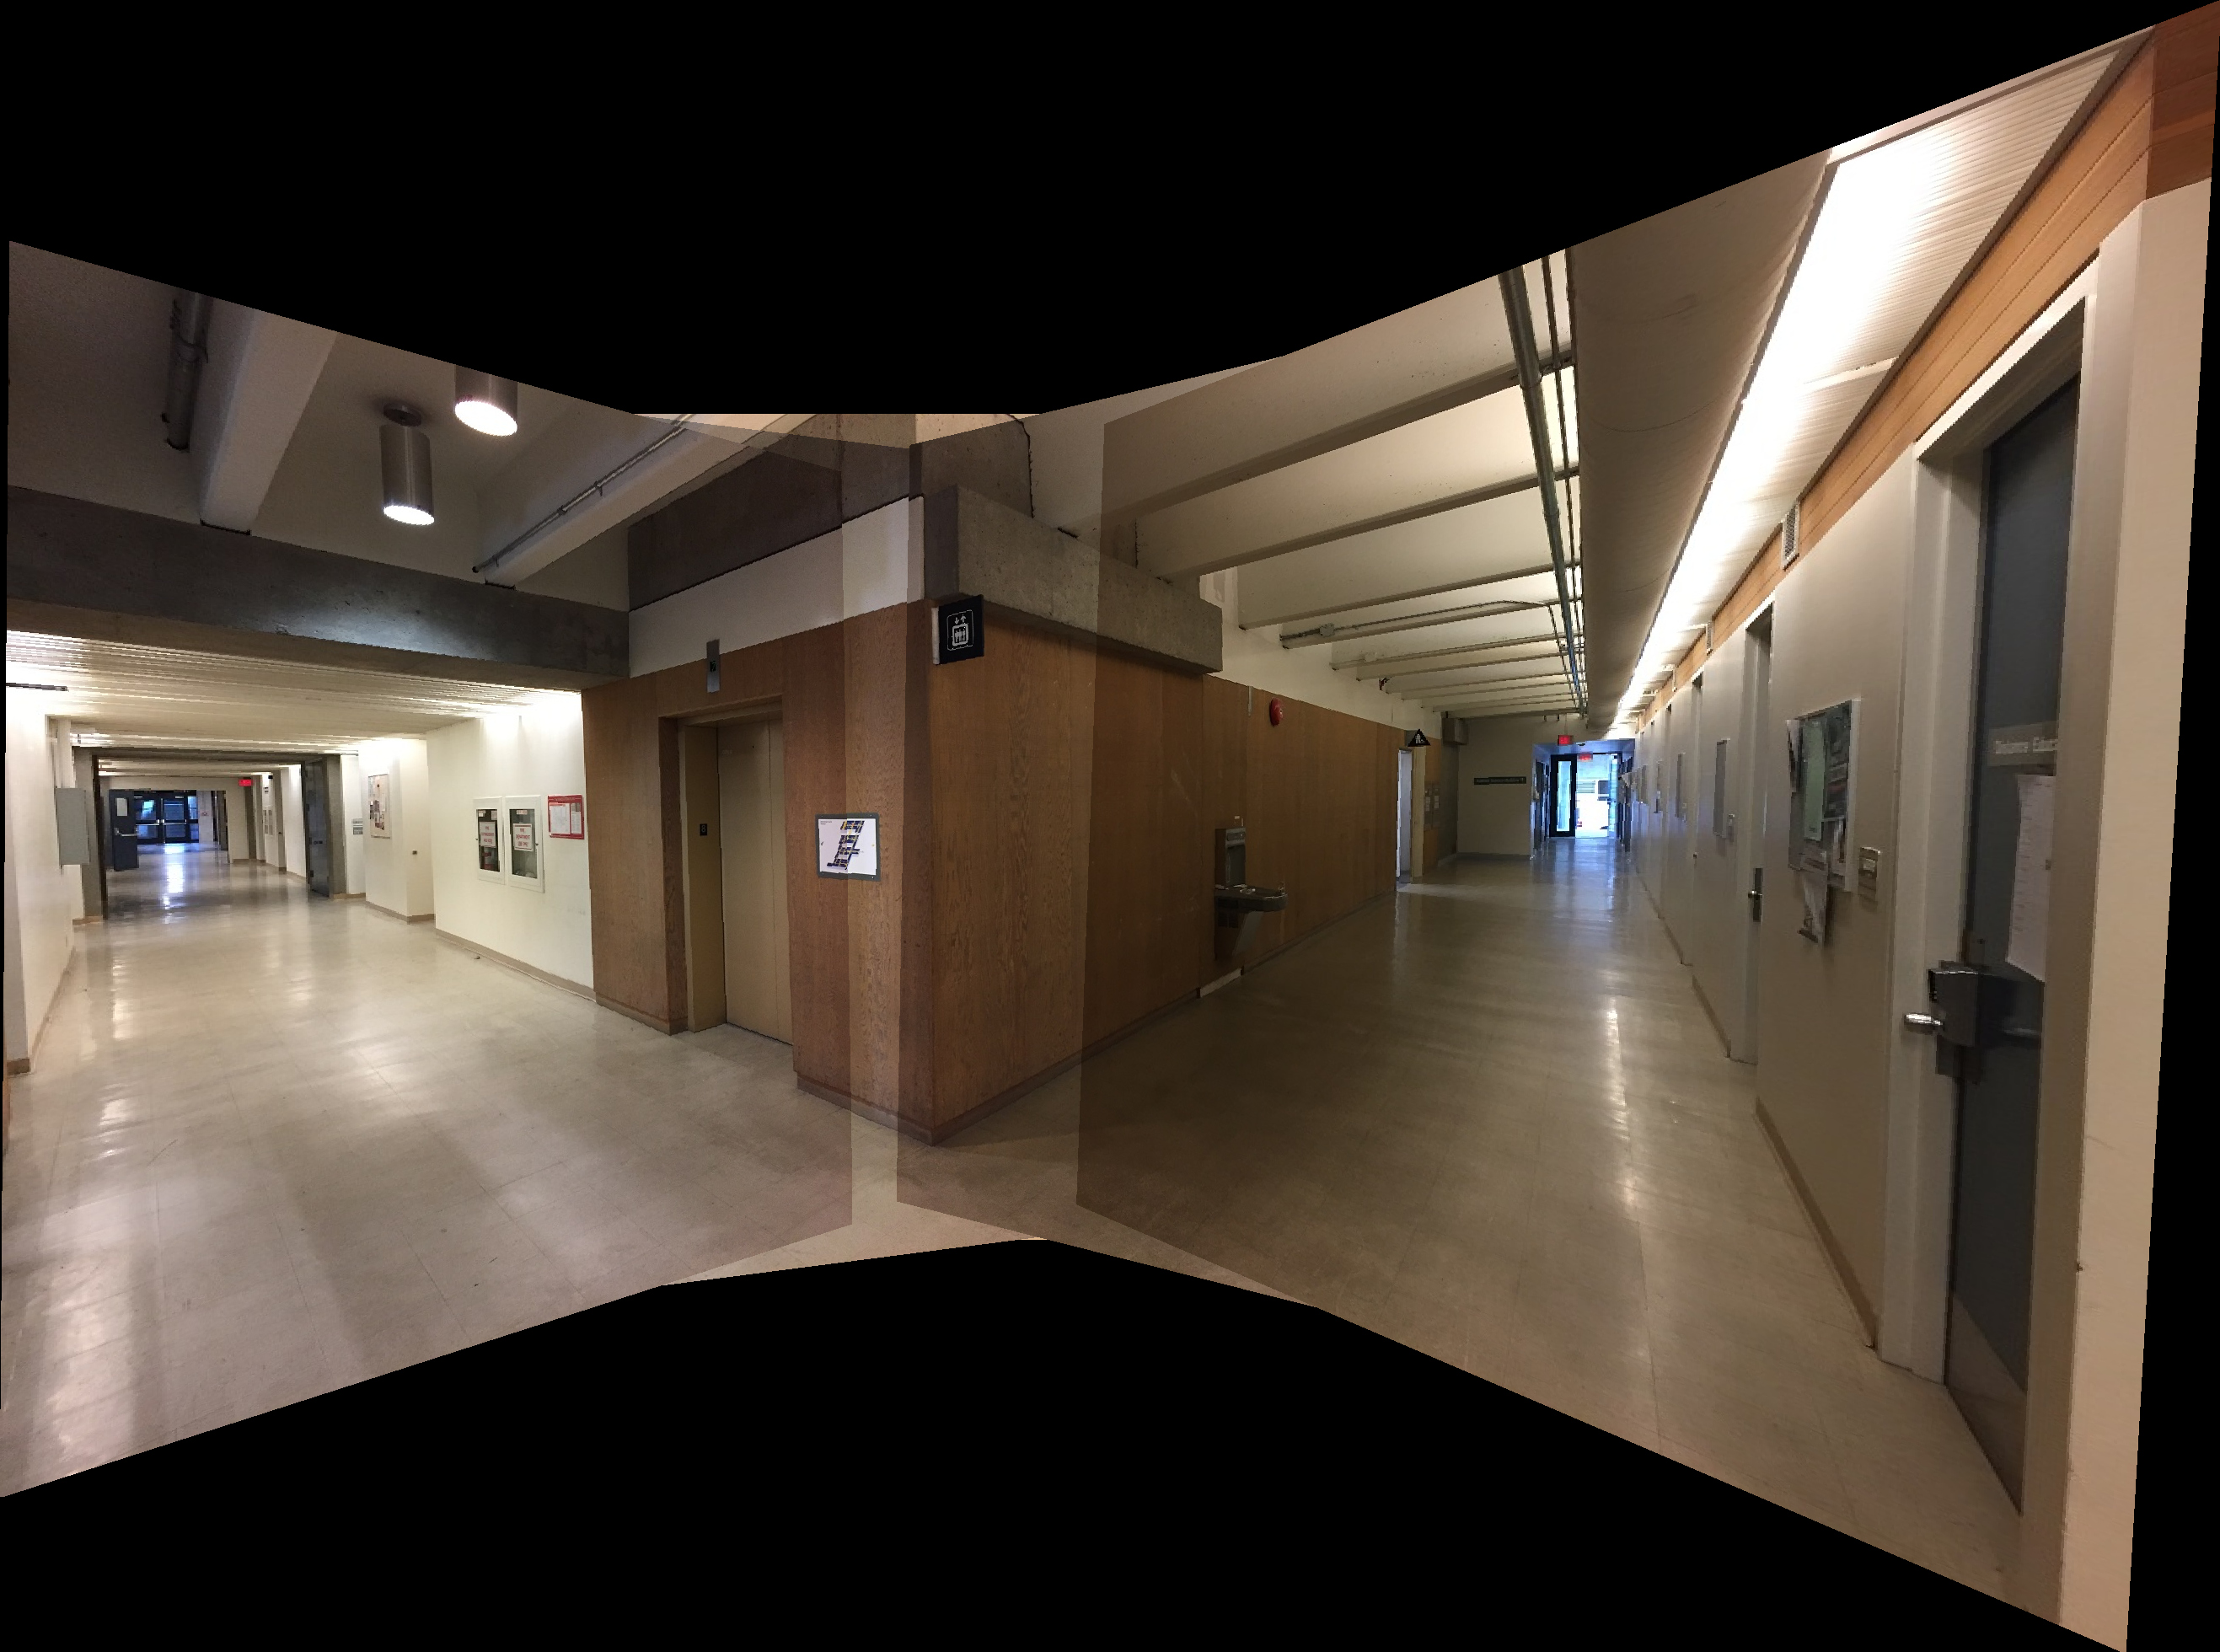
\includegraphics[scale=0.18]{results/p7_noblend/16}
	\centering
	\caption{Unblended version}
\end{figure}
\vspace{300mm}
\begin{figure}[!h]
	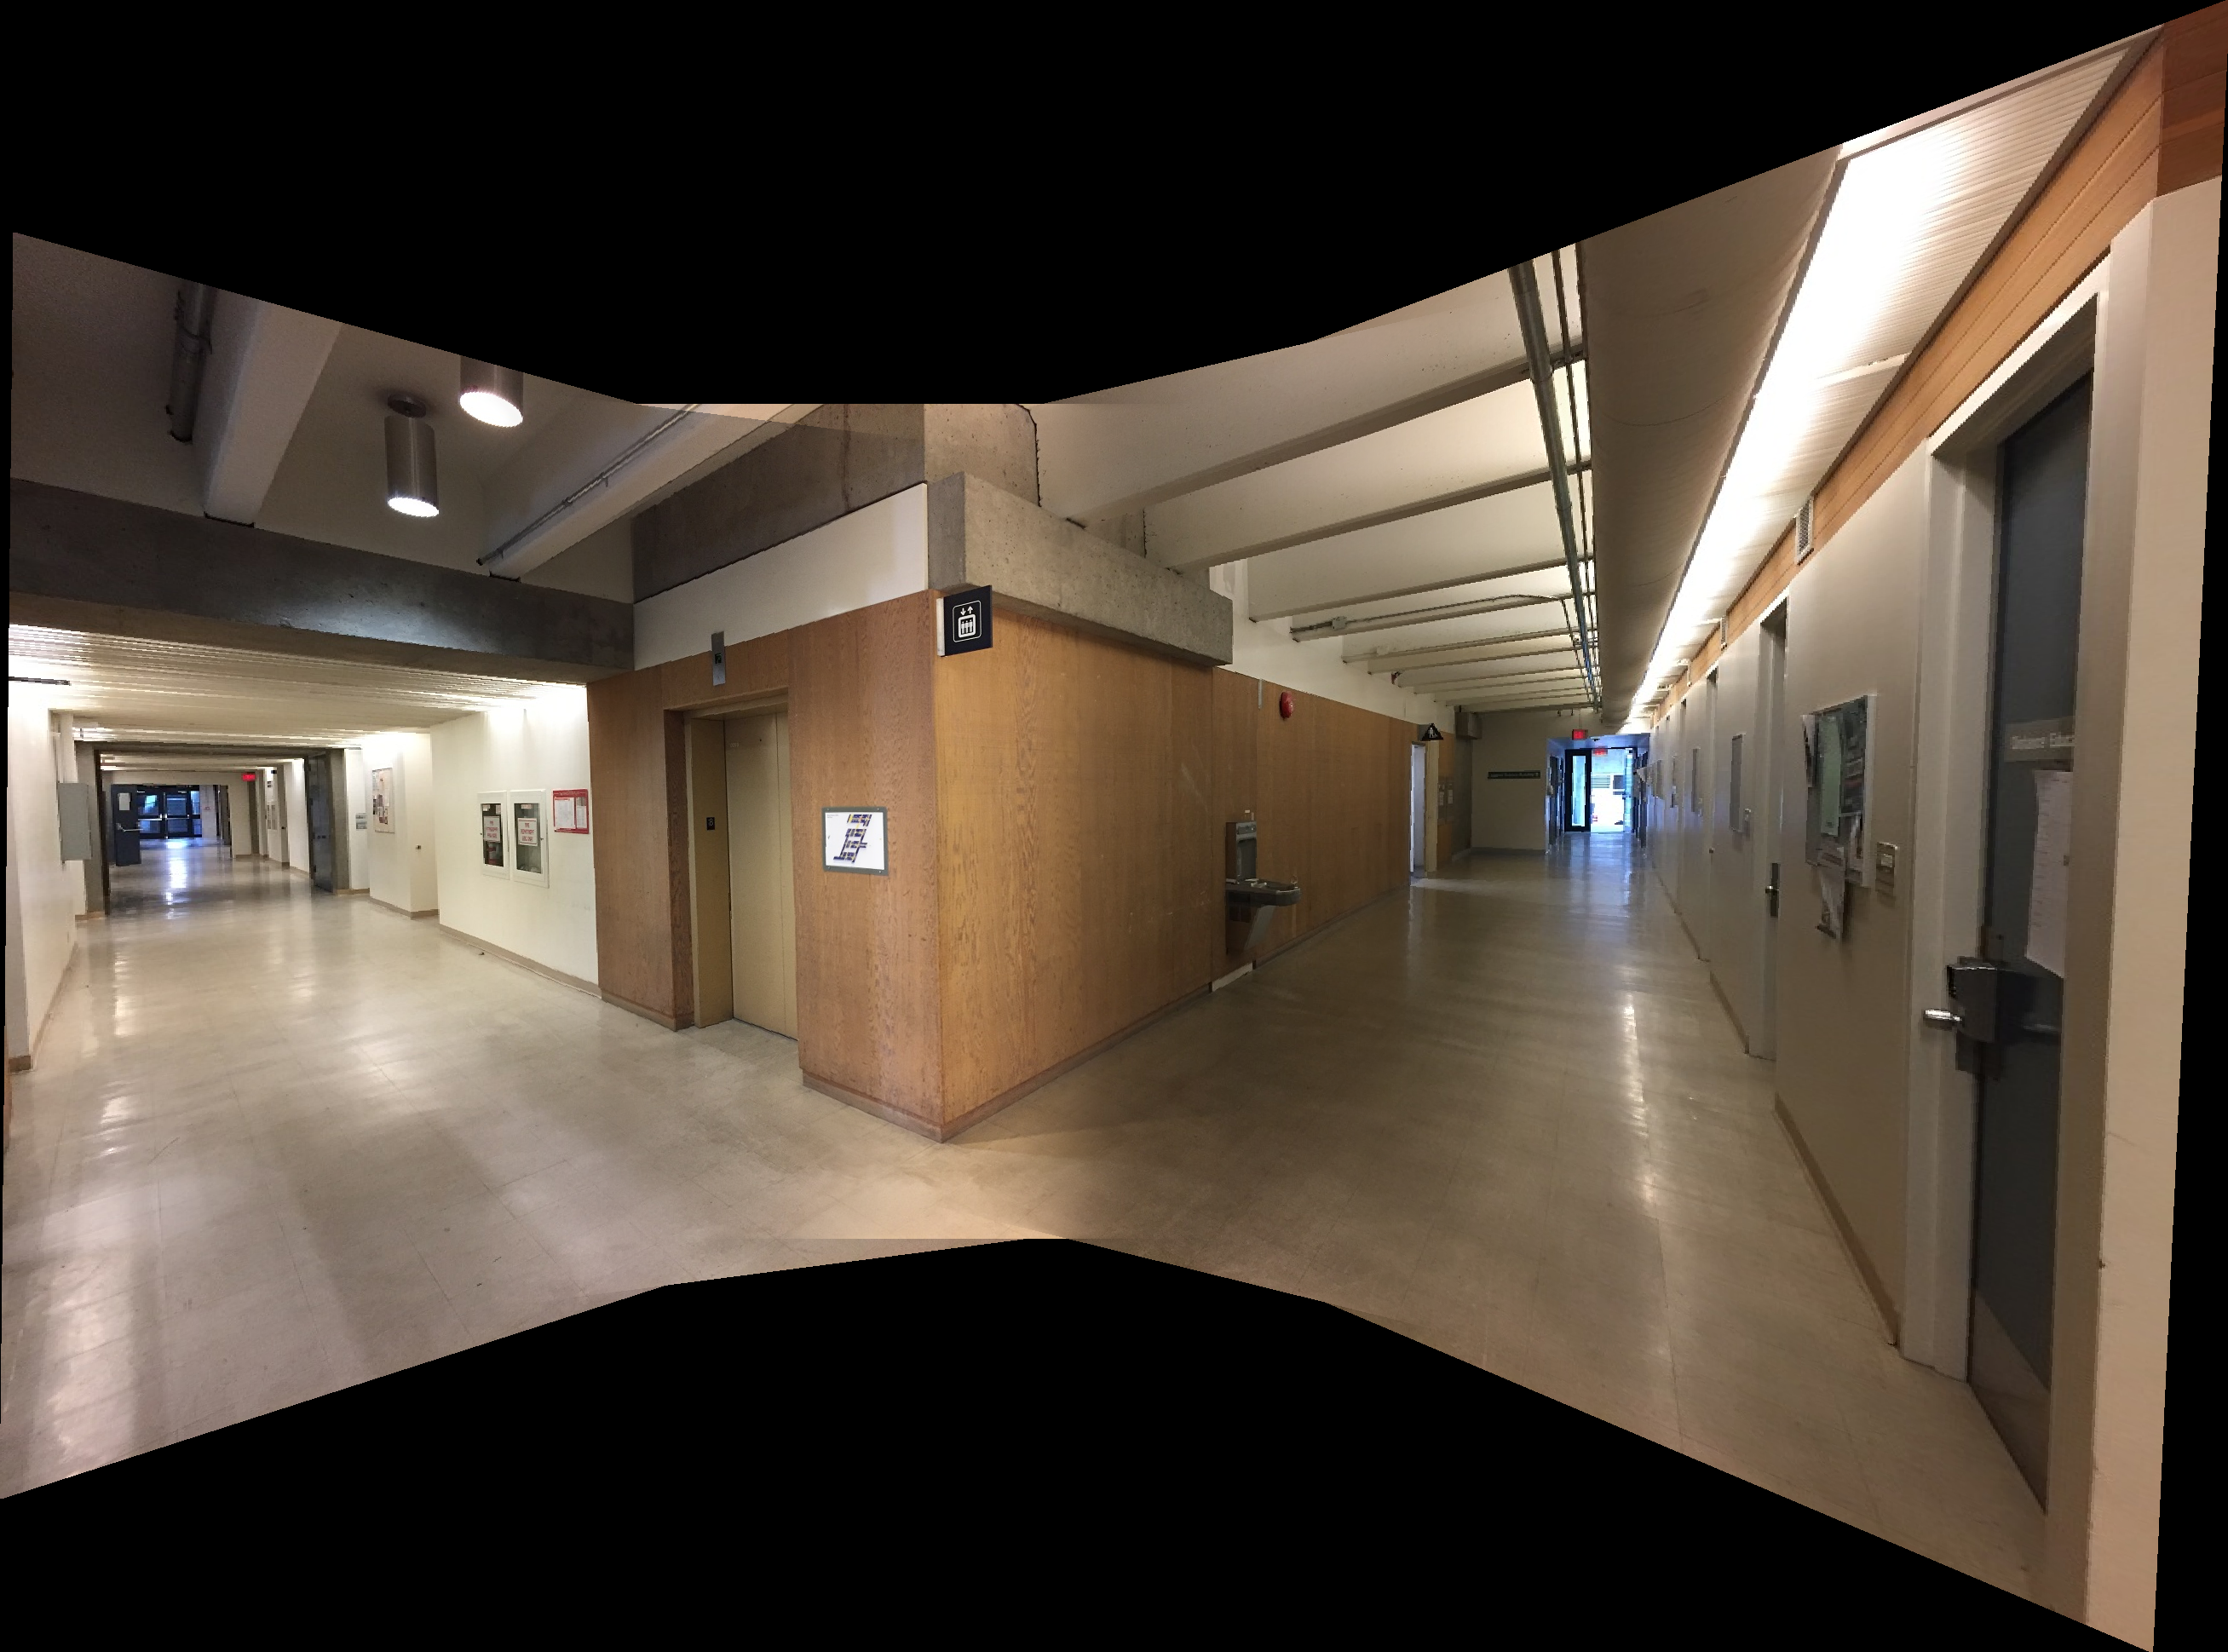
\includegraphics[scale=0.18]{results/p7_blend/16}
	\centering
	\caption{Blended version}
\end{figure}

\begin{figure}[!h]
	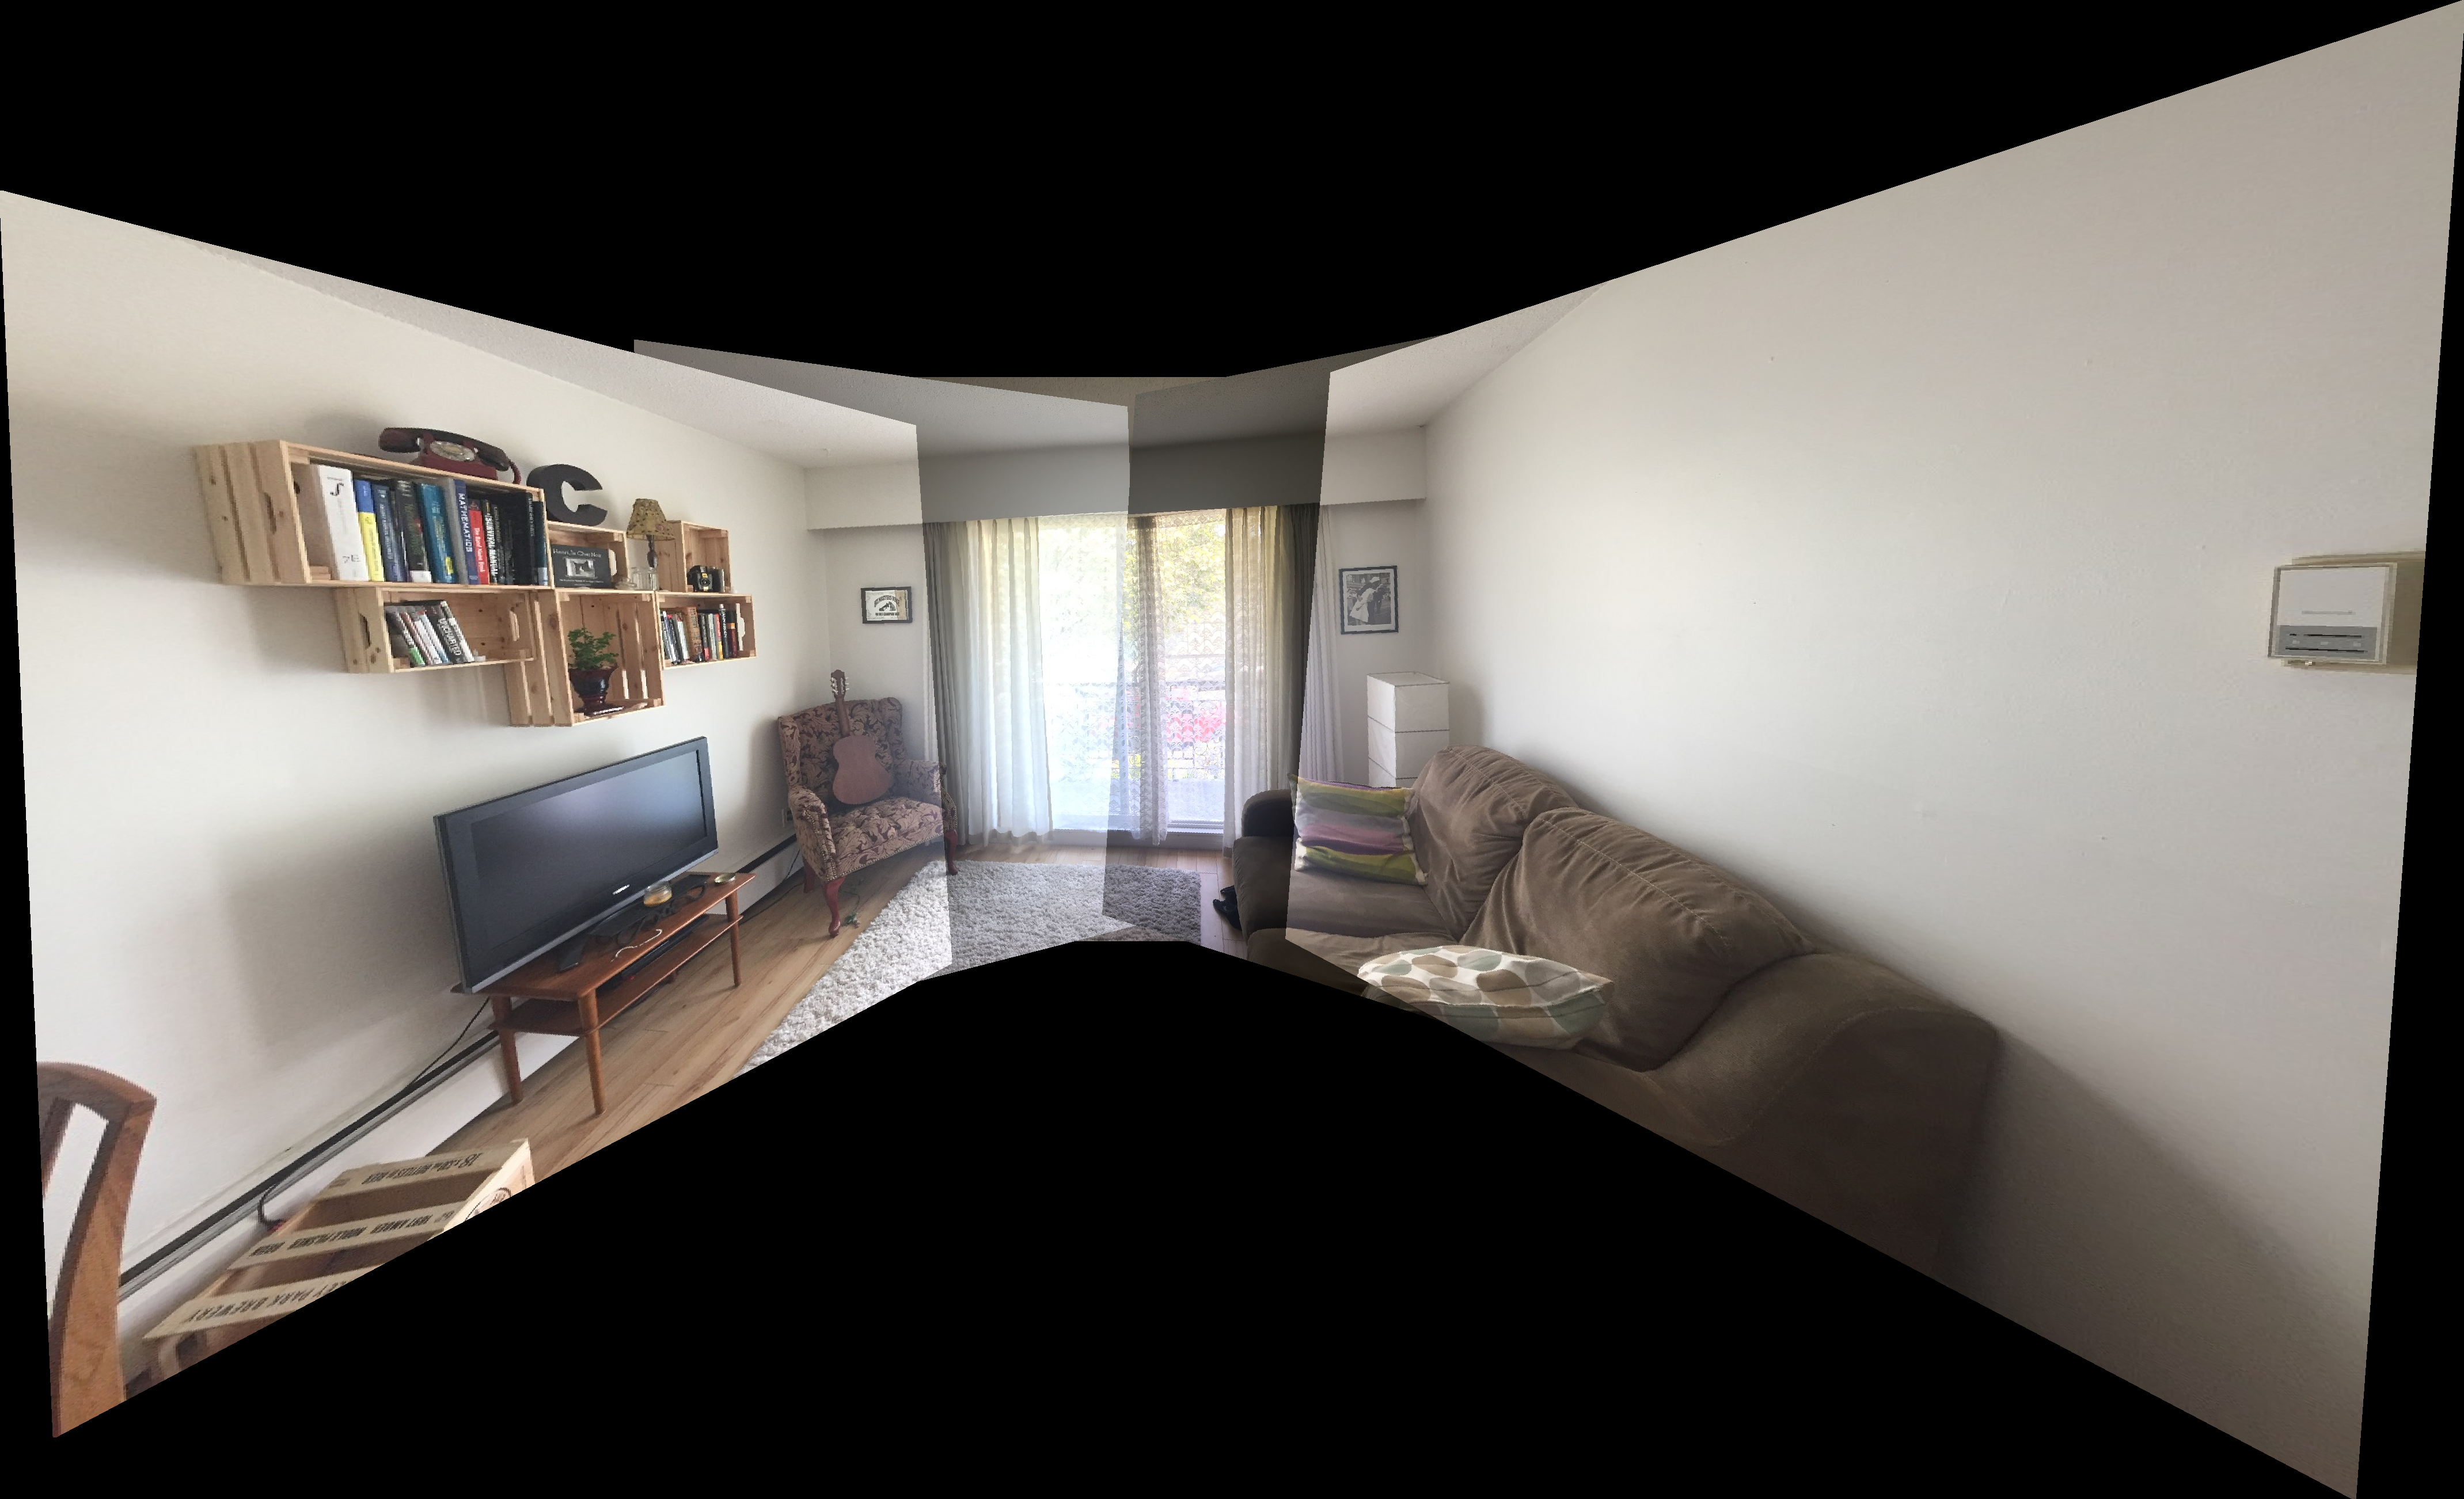
\includegraphics[scale=0.12]{results/p3_noblend/16}
	\centering
	\caption{Unblended version}
\end{figure}
\vspace{100mm}
\begin{figure}[!h]
	\includegraphics[scale=0.12]{results/p3_blend/16}
	\centering
	\caption{Blended version}
\end{figure}

The final result above, although one my favorites, demonstrates the blending issues around the non-overlapping areas of the images. With more time, perhaps other blending techniques would have been explored, but overall I was happy quite with how things turned out.


\end{document}
